\documentclass[a4paper]{article}

%% Language and font encodings
\usepackage[english]{babel}
\usepackage[utf8x]{inputenc}
\usepackage[T1]{fontenc}

%% Sets page size and margins
\usepackage[a4paper,top=3cm,bottom=2cm,left=3cm,right=3cm,marginparwidth=1.75cm]{geometry}

%% Useful packages
\usepackage{amsmath}
\usepackage{amsfonts}
\usepackage{graphicx}
\usepackage[caption=false]{subfig} % subfigures.  false option prevents conflicts in caption styling with other packages
\usepackage{multirow}
\usepackage{multirow}
\usepackage{float}
\usepackage[colorinlistoftodos]{todonotes}
\usepackage[colorlinks=true, allcolors=blue]{hyperref}

%% Custom commands
\newcommand{\DatestampYMD}[3]{\mbox{#1-#2-#3}}
\newcommand{\entry}[3]{\newpage\section*{\DatestampYMD{#1}{#2}{#3}} }

\title{Research Journal}
\author{Stephen Phillips}
\date{June 2018 to Present}

\begin{document}

\maketitle

\entry{2018}{06}{27}
This entry is a bit of catch up, giving some of my initial work and experiments.
\subsection*{Brief High Level Idea}
We are trying to use Graph Neural Networks for feature matching, using cycle consistency as a loss.
What this comes out to in practice is low rank matrix factorization.
However just optimizing typical losses such as the Frobenius norm with a rank loss may not capture real-world noise quite properly.
So the hope is with Neural Nets we can add additional losses to the training for it to incorporate into its factorization at training time, then it will know how to properly do that at testing time.
For now we stick with the aforementioned Frobenius norm to start training.

\subsection*{Literature Review}
\begin{itemize}
\item ``Geometric Deep Learning: Going beyond Euclidean data'' Bronstein et al. 2017.
A survey paper going over many types of non-Euclidean networks.
Here we use the non-fixed structure neural networks.
In particular Kipf and Welling, described below.
\item ``Semi-Supervised Classification with Graph Convolutional Networks'' Kipf and Welling 2017.
This paper takes the graph Laplacian and uses is to multiply a node embedding.
Combine this with weights and non-linearities you have a fully functional neural network.
There was some criticism of this method from \href{https://www.inference.vc/how-powerful-are-graph-convolutions-review-of-kipf-welling-2016-2/}{this blog post} stating that these reduce to rather simple operations when put on a regular graph.
Regardless we will be using this method here.
\item ``The graph neural network model'' Scarselli et al. 2009.
This is a more complicated framework, similar to the previous one but instead using polynomials of the Laplacian instead of just the Laplacian itself.
This gives it more expressively but also means the local nature of it fails to some degree.
This is why I will be using Kipf and Welling as my basis for now.
If that fails, I may try this.
\item ``Relational inductive biases, deep learning, and graph networks'' Battaglia et al. 2018.
This is a high level introduction to a new notion of Graph Neural Networks, with operations on the edges as well as the nodes.
This could be potentially quite helpful but unfortunately there is no implementation of this right now, so using it would be difficult.
For potential future work.
\end{itemize}

\subsection*{Code base}
Initially this was implemented in PyTorch but due to the potential future need for sparse matrices I switched to TensorFlow. The modules of the code are:
\begin{itemize}
\item \texttt{options.py} - This handles all configuration options for building the models, the dataset, and the learning parameters - every other file depends on this one
\item \texttt{model.py} - File with all the models in it - specifically for graph neural networks. All models are sub-classes of \texttt{DenseGraphLayerWeights} which gives a lot of convenience functions for graph networks
\item \texttt{sim\_graphs.py} - Handles synthetic data creation.
\item \texttt{data\_util.py} - Handles generic data creating and loading for graph networks. Has a feature if tensorflow is not able to load it can ignore it and only use Numpy.
\item \texttt{train.py} - Main training file, implements data loading and feeding to neural net pipe-line
\item \texttt{myutils.py} - Lots of convenience functions
\item \texttt{tfutils.py} - Lots of convenience functions but for TensorFlow
\item \texttt{experiment.py} - This is where all the plots are generated. 
\end{itemize}

\subsection*{Exact model}
The input to our neural network is an undirected graph with each node having a starting embedding.
The target is each node having an embedding.
The graph structure is given to us as an $n \times n$ Adjacenty matrix, and the embeddings as an $n \times m$ matrix $E$ (typically $m << n$).
Thus using Kipf and Welling as our guide, we have our update rule for layer $i$ as:
\begin{align*}
D = \mathrm{diag}((A + I) \mathbf{1}) \\
L = D^{-1/2}(A + I)D^{-1/2} \\
E_{i+1} = \sigma \left(LE_{i} W^{(i+1)}\right) + E_{i} U^{(i+1)}
\end{align*}
With $W^{(i+1)}$ and $U^{(i+1)}$ being a $m_i \times m_{i+1}$ matrix, and $E_i$ being a $n \times m_i$ matrix (with $E_0 = E$).
$\sigma$ here is our non-linearity.
The $U$ weights are for skip connections.
The final layer $F$ is each row of the final embedding $E_N$ normalized to norm 1 (here our network has $N$ layers).

This model seems reasonable.
Consider the special case if $m_i = 1$ for all $i$ and $\sigma(x) = x / \|x\|$.
Setting the weights to be 1, we get $E_{i+1} = L E_i / \| L E_i \|$.
This is exactly the power method of finding the leading eigenvectors, which is an approximation of cycle consistency.

\subsection*{Experiments}
First this was generated using 3 random $25 \times 25$ permutation matrices stacked together to form a $75 \times 25$  matrix as the ground truth node embedding vectors $E_{gt}$, then using the outer product to make a $75 \times 75$ matrix $S_{gt} = E_{gt} E_{gt}^\top$, which serves as the ground truth graph.
We have some noise function $\nu$ and so the given graph is $A = \nu(E_{gt})$.
We get our output embedding $F$ So this is essentially testing if we can do matrix factorization via Graph Neural Networks with various noise models.
We have a very noisy initial embedding.
To compute the error, we compute the factored similarity matrix, which means we normalize each embedding row then do an outer product.
For the figures we display the node embedding vectors grouped by the ground truth labels, so the true plots look like a diagonal matrix.

% Figure \ref{fig:baseline_plot} shows an example of ground truth node embedding and similarities as well as the node embedding vectors and similarities of the initial embedding we use.
% 
\begin{figure}[H]
    \centering
    % \includegraphics[width=0.7\textwidth]{figures/noiseless_sim.png}
    \begin{minipage}{.45\linewidth}
        \subfloat[Sorted ground truth embedding and initial embedding]{ 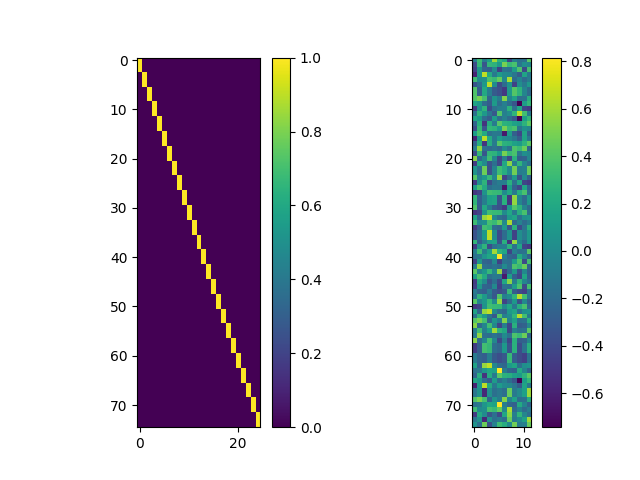
\includegraphics[width=0.9\textwidth]{figures/baseline_embeddings.png} \label{fig:baseline_sub1} }
    \end{minipage}
    \begin{minipage}{.45\linewidth}
        \subfloat[Ground truth and initial similarity]{ 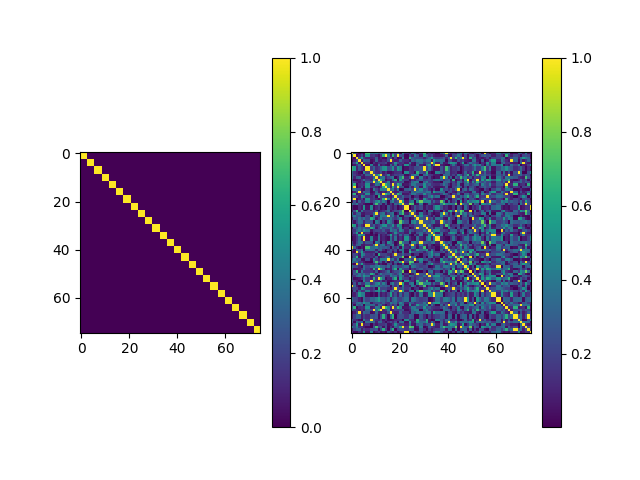
\includegraphics[width=0.9\textwidth]{figures/baseline_sim.png} \label{fig:baseline_sub2} }
    \end{minipage}
    \caption{Here we show a baseline for the node embedding vectors and the final similarity matrix}
    \label{fig:baseline_plot}
\end{figure}

\subsubsection*{Noiseless Dataset}
Here we use no noise to distort it.
This is equivalent to see if Neural Networks can do matrix factorization on a truly low rank matrix.
\begin{figure}[H]
    \centering
    % \includegraphics[width=0.7\textwidth]{figures/noiseless_sim.png}
    \subfloat[Typical embedding and similarity matrix of Noiseless]{ 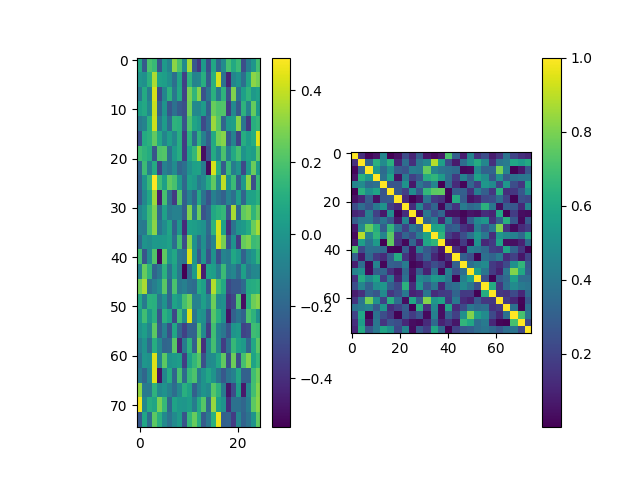
\includegraphics[width=0.45\textwidth]{figures/synth_plot.png} \label{fig:noiseless_sub1} }
    \subfloat[Typical histogram for similarities of noiseless]{ 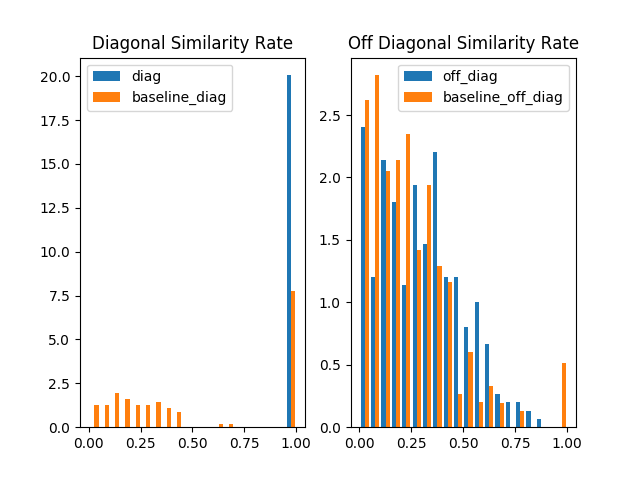
\includegraphics[width=0.45\textwidth]{figures/synth_hist.png} \label{fig:noiseless_sub2} }
    \caption{Here we show a baseline for the node embedding vectors and the final similarity matrix}
    \label{fig:noiseless_plot}
\end{figure}
The numerical scores come out to be:
\begin{table}[H]
    \centering
    \begin{tabular}{|c|c|} \hline
        Trained Same Point Similarity      & 1.00e+00 $\pm$ 8.07e-08  \\ \hline
        Trained Distinct Point Similarity  & 2.81e-01 $\pm$ 1.81e-01  \\ \hline
        Baseline Same Point Similarity     & 5.04e-01 $\pm$ 3.89e-01  \\ \hline
        Baseline Distinct Point Similarity & 2.56e-01 $\pm$ 2.06e-01  \\ \hline
    \end{tabular}
    \caption{Average cross similarity between points, for no noise}
    \label{tab:noiseless_table}
\end{table}

\subsubsection*{Pairwise Matrix Multiplication Noise}
Our noise model for this one $\nu$ is described by, for the block in row $i$, column $j$
\begin{equation*}
    \nu(E)_{ij} = E_i N_{ij} E_j^\top, \quad \quad N_{ij} = \theta I + (1-\theta) \sum_{k=1}^K M_{ij}^k , \quad \quad M_{ij}^{k} \sim {\Pi}(m, m)
\end{equation*}
With the constraint that $N_{ij} = N_{ji}^\top$.
Here $\Pi(m,m)$ denotes the uniform distribution over the $m \times m$ permutation matrices, and $\theta$, and $K$ are parameters.

\paragraph{Parameter Set 1}
Here, $\theta = 0.9$, $K = 1$.
\begin{figure}[H]
    \centering
    % \includegraphics[width=0.7\textwidth]{figures/noiseless_sim.png}
    \subfloat[Typical embedding and similarity matrix of pairwise noise]{ 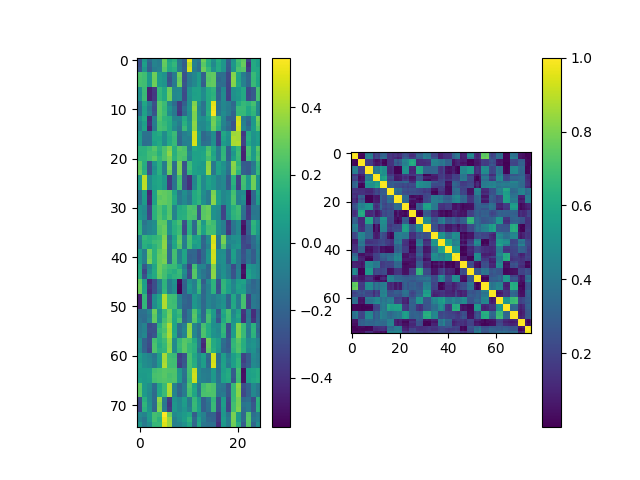
\includegraphics[width=0.45\textwidth]{figures/pairwise_plot.png} \label{fig:pairwise_sub1} }
    \subfloat[Typical histogram for similarities of pairwise noise]{ 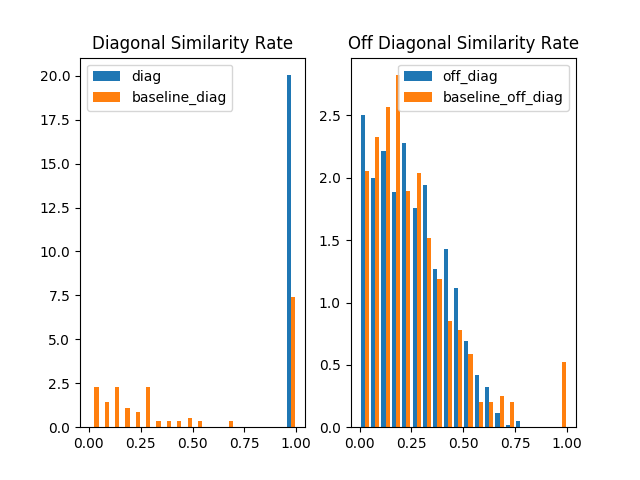
\includegraphics[width=0.45\textwidth]{figures/pairwise_hist.png} \label{fig:pairwise_sub2} }
    \caption{Here we show a baseline for the node embedding vectors and the final similarity matrix}
    \label{fig:pairwise_plot}
\end{figure}
Note the clear separation between diagonal and off diagonal in the histogram. The numerical scores come out to be: 
\begin{table}[H]
    \centering
    \begin{tabular}{|c|c|} \hline
        Trained Same Point Similarity      & 9.97e-01 $\pm$ 4.62e-03  \\ \hline
        Trained Distinct Point Similarity  & 2.86e-01 $\pm$ 1.76e-01  \\ \hline
        Baseline Same Point Similarity     & 5.12e-01 $\pm$ 3.90e-01  \\ \hline
        Baseline Distinct Point Similarity & 2.56e-01 $\pm$ 2.06e-01  \\ \hline
    \end{tabular}
    \caption{Average cross similarity between points, for pairwise noise with $K=1$}
    \label{tab:pairwise_table}
\end{table}

\paragraph{Parameter Set 2}
Here, $\theta = 0.9$, $K = 3$.
\begin{figure}[H]
    \centering
    % \includegraphics[width=0.7\textwidth]{figures/noiseless_sim.png}
    \subfloat[Typical embedding and similarity matrix of pairwise noise]{ 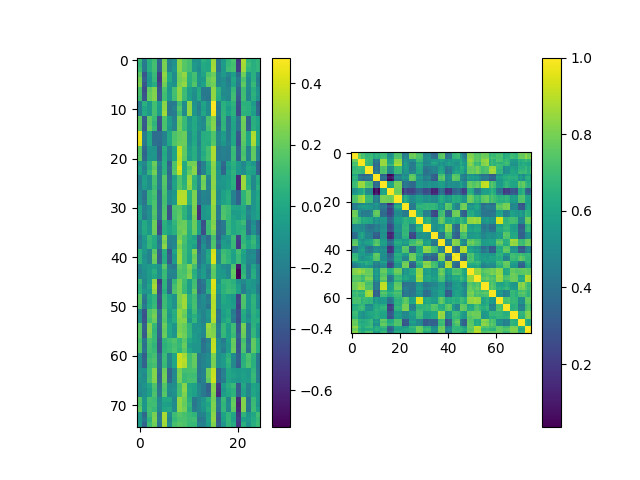
\includegraphics[width=0.45\textwidth]{figures/pairwise3_plot.png} \label{fig:pairwise3_sub1} }
    \subfloat[Typical histogram for similarities of pairwise noise]{ 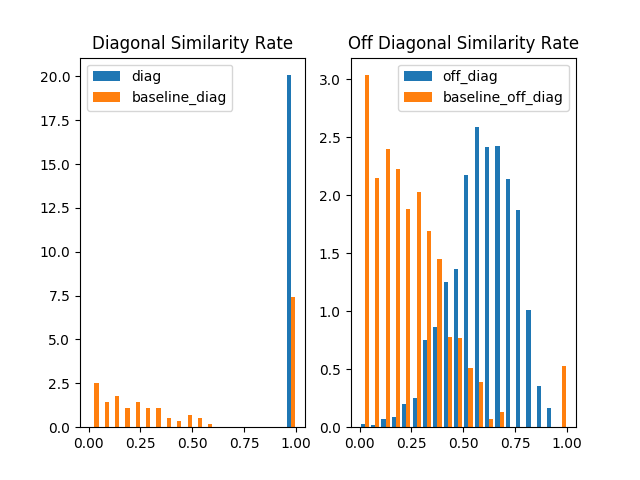
\includegraphics[width=0.45\textwidth]{figures/pairwise3_hist.png} \label{fig:pairwise3_sub2} }
    \caption{Here we show a baseline for the node embedding vectors and the final similarity matrix}
    \label{fig:pairwise3_plot}
\end{figure}
Note that the diagonal and off diagonal entries overlap quite a bit.
The numerical scores come out to be:
\begin{table}[H]
    \centering
    \begin{tabular}{|c|c|} \hline
        Trained Same Point Similarity      & 9.96e-01 $\pm$ 6.24e-03  \\ \hline
        Trained Distinct Point Similarity  & 6.35e-01 $\pm$ 1.42e-01  \\ \hline
    \end{tabular}
    \caption{Average cross similarity between points, for pairwise noise with $K=3$}
    \label{tab:pairwise3_table}
\end{table}

\paragraph{Parameter Set 3}
Here, $\theta = 0.9$, $K = 5$.
\begin{figure}[H]
    \centering
    % \includegraphics[width=0.7\textwidth]{figures/noiseless_sim.png}
    \subfloat[Typical embedding and similarity matrix of pairwise noise]{ 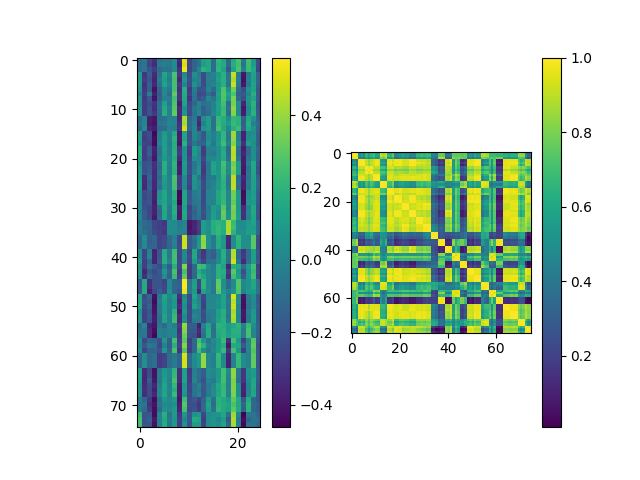
\includegraphics[width=0.45\textwidth]{figures/pairwise5_plot.png} \label{fig:pairwise5_sub1} }
    \subfloat[Typical histogram for similarities of pairwise noise]{ 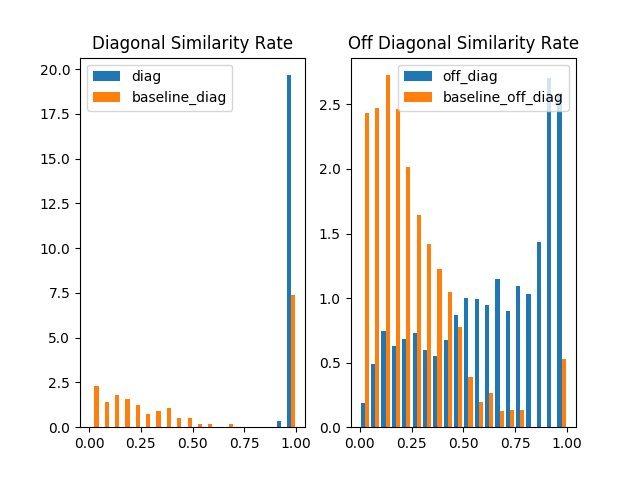
\includegraphics[width=0.45\textwidth]{figures/pairwise5_hist.png} \label{fig:pairwise5_sub2} }
    \caption{Here we show a baseline for the node embedding vectors and the final similarity matrix}
    \label{fig:pairwise5_plot}
\end{figure}
Note that the diagonal and off diagonal entries overlap almost completely.
There is something that goes wrong, and I need to do more investigation before I can determine why.
The numerical scores come out to be:
\begin{table}[H]
    \centering
    \begin{tabular}{|c|c|} \hline
        Trained Same Point Similarity      & 9.90e-01 $\pm$ 2.54e-02  \\ \hline
        Trained Distinct Point Similarity  & 5.82e-01 $\pm$ 3.91e-01  \\ \hline
    \end{tabular}
    \caption{Average cross similarity between points, for pairwise noise with $K=5$}
    \label{tab:pairwise5_table}
\end{table}

\entry{2018}{06}{27}
\subsection*{Larger Dataset Test}
So I was considering that the poor performance might have something to do with overfitting so I decided, since this is synthetic data to generate many more samples in the dataset.
I got the following results for the $K=3$, slightly better than before but within noise.
To put a nail in this coffin, I have been working on generating samples on the fly for training, giving effectively infinite data.
Here are the current results, $\theta = 0.9$, $K = 3$.
\begin{figure}[H]
    \begin{minipage}{.45\linewidth}
        \centering
        \subfloat[Typical embedding and similarity matrix of pairwise noise]{ 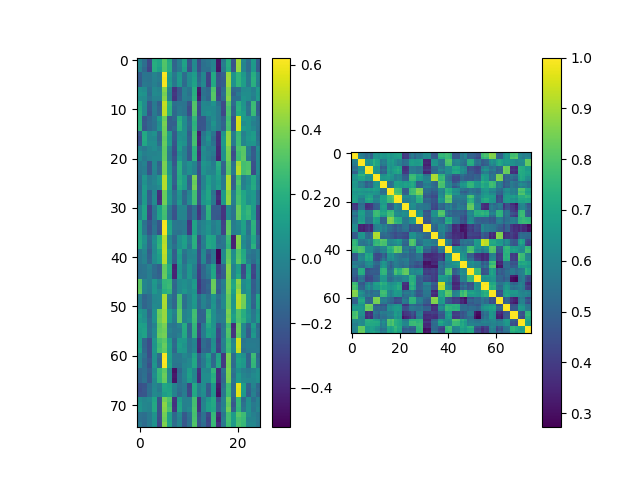
\includegraphics[width=0.9\textwidth]{figures/pairwise3_large_plot.png} \label{fig:pairwise3_large_sub1} }
    \end{minipage}
    \begin{minipage}{.45\linewidth}
        \centering
        \subfloat[Typical histogram for similarities of pairwise noise]{ 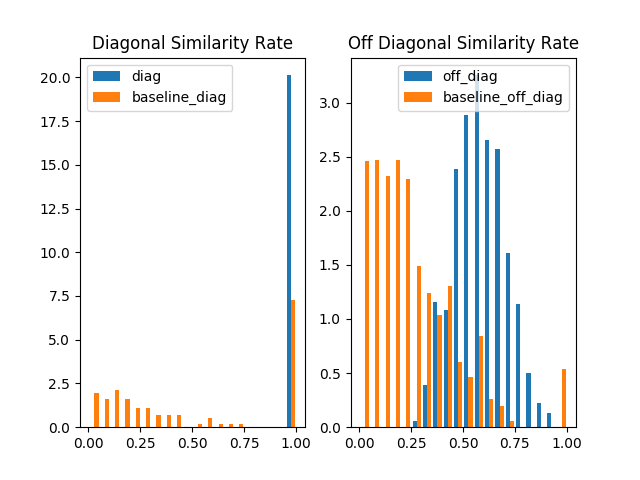
\includegraphics[width=0.9\textwidth]{figures/pairwise3_large_hist.png} \label{fig:pairwise3_large_sub2} }
    \end{minipage}
    \centering
    \subfloat[Numerical results]{
        \begin{tabular}{|c|c|c|c|} \hline
                                       &    Trained Model        &    Previous Model        &    Baseline             \\ \hline
            Same Point Similarity      & 9.97e-01 $\pm$ 4.16e-03 & 9.96e-01 $\pm$ 6.24e-03 & 5.11e-01 $\pm$ 3.91e-01 \\ \hline
            Distinct Point Similarity  & 6.34e-01 $\pm$ 1.29e-01 & 6.35e-01 $\pm$ 1.42e-01 & 2.55e-01 $\pm$ 2.06e-01  \\ \hline
        \end{tabular}
        \label{fig:pairwise3_large_tab1}
    }
    \label{fig:pairwise3_large_plot}
\end{figure}

\entry{2018}{07}{02}
\subsection*{Infinite Dataset Test}
After much debugging to get the data generation during training working, we managed to run some experiments.
Testing with infinite data did seem to improve generalization substantially compared to a simply larger dataset.
So it seems that data is in fact a problem, we will somehow have to address this. 
This is run on the pairwise dataset with $K=3$.
\begin{figure}[H]
    \begin{minipage}{.45\linewidth}
        \centering
        \subfloat[Typical embedding and similarity matrix of pairwise noise]{ 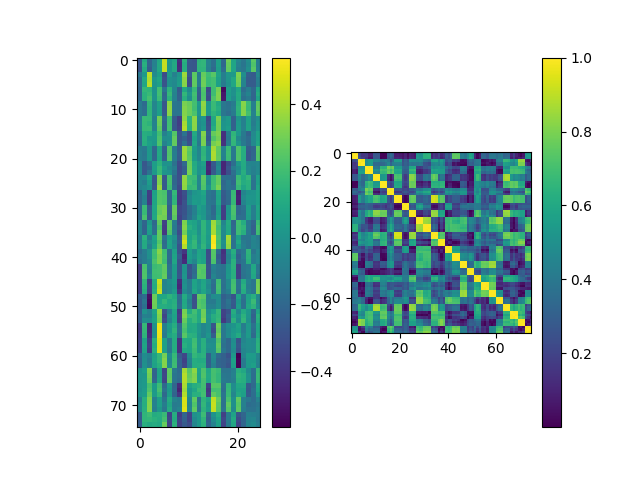
\includegraphics[width=0.9\textwidth]{figures/pairwise3inf_plot.png} \label{fig:pairwise3inf_sub1} }
    \end{minipage}
    \begin{minipage}{.45\linewidth}
        \centering
        \subfloat[Typical histogram for similarities of pairwise noise]{ 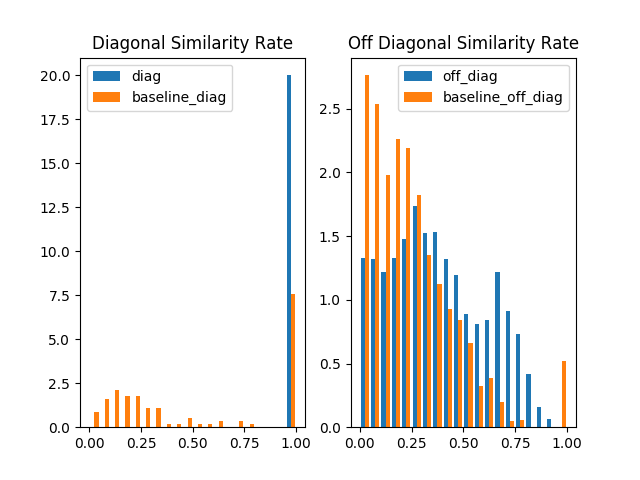
\includegraphics[width=0.9\textwidth]{figures/pairwise3inf_hist.png} \label{fig:pairwise3inf_sub2} }
    \end{minipage}
    \centering
    \subfloat[Numerical results]{
        \begin{tabular}{|c|c|c|c|} \hline
                                       &    Trained Model        &    Previous Model        &    Baseline             \\ \hline
            Same Point Similarity      & 9.96e-01 $\pm$ 5.22e-03 & 9.97e-01 $\pm$ 4.16e-03 & 5.11e-01 $\pm$ 3.91e-01 \\ \hline
            Distinct Point Similarity  & 4.31e-01 $\pm$ 2.15e-01 & 6.34e-01 $\pm$ 1.29e-01 & 2.55e-01 $\pm$ 2.06e-01  \\ \hline
        \end{tabular}
        \label{fig:pairwise3inf_large_tab1}
    }
    \label{fig:pairwise3inf_plot}
\end{figure}
Despite this, the distinction between diagonal and off diagonal entries is not as sharp as I would like.
I need to brainstorm ideas of how to handle that.
There is some work on doing better selection for which edges in the averaging are relevant (e.g. Graph Attention Networks)

\entry{2018}{07}{03}
\subsection*{Infinite Dataset Test}
I ran more experiments with the infinite dataset but with a harder dataset.
This is run on the pairwise dataset with $K=5$.
\begin{figure}[H]
    \begin{minipage}{.45\linewidth}
        \centering
        \subfloat[Typical embedding and similarity matrix of pairwise noise]{ 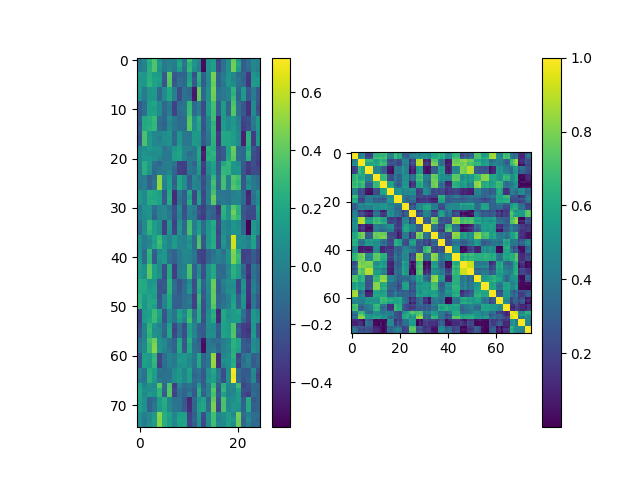
\includegraphics[width=0.9\textwidth]{figures/pairwise5inf_plot.png} \label{fig:pairwise5inf_sub1} }
    \end{minipage}
    \begin{minipage}{.45\linewidth}
        \centering
        \subfloat[For comparison, the non-infinite data trained version]{ 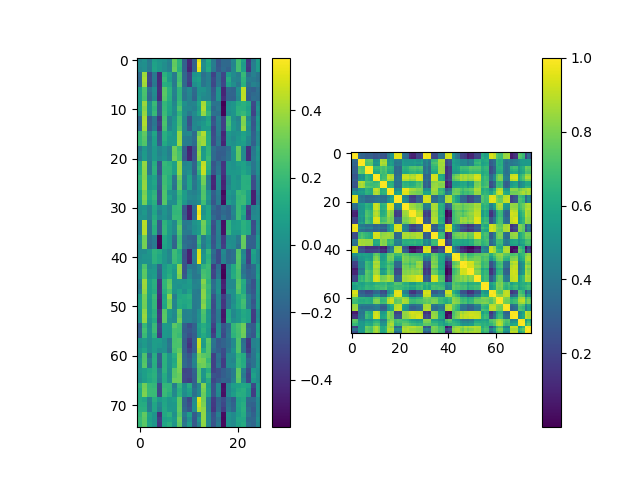
\includegraphics[width=0.9\textwidth]{figures/pairwise5inf_plot_compare.png} \label{fig:pairwise5inf_sub2} }
    \end{minipage}
    \begin{minipage}{.9\linewidth}
        \centering
        \subfloat[Typical histogram for similarities of pairwise noise]{ 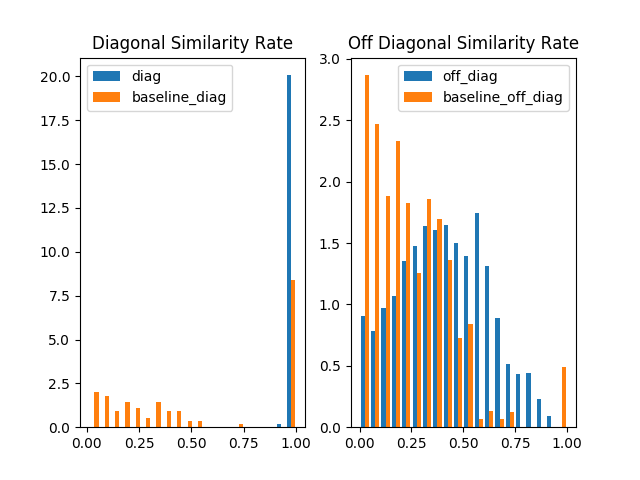
\includegraphics[width=0.5\textwidth]{figures/pairwise5inf_hist.png} \label{fig:pairwise5inf_sub3} }
    \end{minipage}
    \centering
    \subfloat[Numerical results]{
        \begin{tabular}{|c|c|c|c|} \hline
                                       &    Trained Model        &    Previous Model        &    Baseline             \\ \hline
            Same Point Similarity      & 9.97e-01 $\pm$ 3.70e-03 & 9.96e-01 $\pm$ 5.38e-03 & 5.11e-01 $\pm$ 3.91e-01 \\ \hline
            Distinct Point Similarity  & 6.71e-01 $\pm$ 1.55e-01 & 7.13e-01 $\pm$ 1.59e-01 & 2.55e-01 $\pm$ 2.06e-01  \\ \hline
        \end{tabular}
        \label{fig:pairwise5inf_tab1}
    }
    \label{fig:pairwise3inf_large_plot}
\end{figure}
It does OK, but this is still a fairly weak noise model even with the stronger noise.
If the noise got more intense, we would need additional mechanisms to handle it.
Hence the next mechanism.

\subsection*{Graph Attention Network Code Review}
I was looking at the aforementioned Graph Attention Network (GAT) \href{https://arxiv.org/pdf/1710.10903.pdf}{paper} and its \href{https://github.com/PetarV-/GAT}{code}.

\entry{2018}{07}{04}
\subsection*{GAT Implementation details}
After careful looking at the paper and the code for the GAT paper.
After some confusing reading of the code, I figured out the way they are actually implementing it.
It is more naive than I originally thought unfortunately.
Let $E_k$ be the node embedding vectors at the current layer, with adjacency matrix $A$, and weight matrices $T_{k,1}, T_{k,2} \in \mathbb{R}^{n_k \times m_k}$, with $l$ being a point-wise non-linear function, and $s$ being the row-wise-softmax function:
\begin{align*}
f_1 =&\; E_k T_{k,1} \\
f_2 =&\; E_k T_{k,2} \\
Q_k =&\; l(f_1 So \mathbf{1}^\top + \mathbf{1} f_2^\top) \\
E_{k+1} =&\; \sigma \left( s(Q_k + A) E_k W_k \right)
\end{align*}
This has a few problems - This method is really dense.
They have a sparse method but it computes this densely then makes it sparse.
Also if you wanted to enforce the symmetry of the weights on the graph.
. there isn't really a simple way to do that.
Except maybe doing something like using $Q_k' = (Q_k + Q_k^\top)/2$ which doesn't help the whole sparsity problem.
There are some simple ways to make this sparse using for loops but I am uncertain how to do this using TensorFlow... or even PyTorch.
However, as I don't see another way to learn the weights of the edges, this is what I'll be focusing on. 

\subsection*{Leaky ReLU Experiments}
So inspired by the previous paper I thought I would try running experiments with the Leaky ReLU nonlinearity, just to see if it was any different.
As it turns out, unsurprisingly, not too much.

\entry{2018}{07}{05}
\subsection*{Binary Cross Entropy}
Talking with others in the lab (Drew, Oleh) I realized instead of the L2 loss perhaps the Binary Cross Entropy (BCE) Loss would perform better.
Unfortunately this would make it less directly comparable to the optimization methods, but still I think it would worth trying.
First I need to change the datasets to make sure that they don't go over weight 1, which means regeneration of all the datasets.
Next I have to add an addtional loss option for choosing between L2 loss and BCE loss.

\subsection*{TensorFlow Implementation Details}
So my TensorFlow code is OK but it lacks some nice features.
Talking to Drew, it seems Sonnet is the answer, since he showed me some of the features I was missing.
I also need to start using \texttt{SingularMonitoredSession} instead of slim since slim is just... annoying.
So I will need to branch off in git and make a new branch while I get Sonnet working.

\entry{2018}{07}{09}
\subsection*{TensorFlow Implementation Details}
Still working on updating the TensorFlow features to use Sonnet.

\entry{2018}{09}{17}
I have much ground to catch up on. But better late than never.
\subsection*{TensorFlow Implementation Details Completed}
I finished this and the code is much cleaner - the code is divided better. The \texttt{model.py} function has been replaced with a model module (directory with multiple files), so now custom layers, custom network types, and the architecture selection logic are separated. However, the regularization is still a bit crude, and when building a new architecture it tends to give a 'gotcha' - I need to fix that. Otherwise it is working much better.
\subsection*{Binary Cross Entropy afterthoughts}
I have not tested this extensively but the limited experiments I did try didn't seem to make much of a difference. I think it might be better dealing with outliers. Right now we use a Frobenious norm loss, which implicitly assumes $A_{ij} \sim \mathcal{N}(e_i^\top e_j, \sigma^2)$. This assumes infinte support and is not quite we are assuming if we enforce $e_i$ to be norm 1. Thus the rational is since it is between 0 and 1, we can treat each element as a classifcation: $P(A_{ij} = 1) = 1 - P(A_{ij} = 0) = e_i^\top e_j$. This is more appropriate and possibly more robust to noise (maybe outliers?). However, more tests need to be done to determine its actual effectiveness.
\subsection*{Experiments}
Many experiments were done during this time. Here are the tables and figures

\subsubsection*{Experiment Run 12}
Dataset type $\texttt{synth3view}$ - noiseless 3 view dataset.

\begin{figure}[H]
  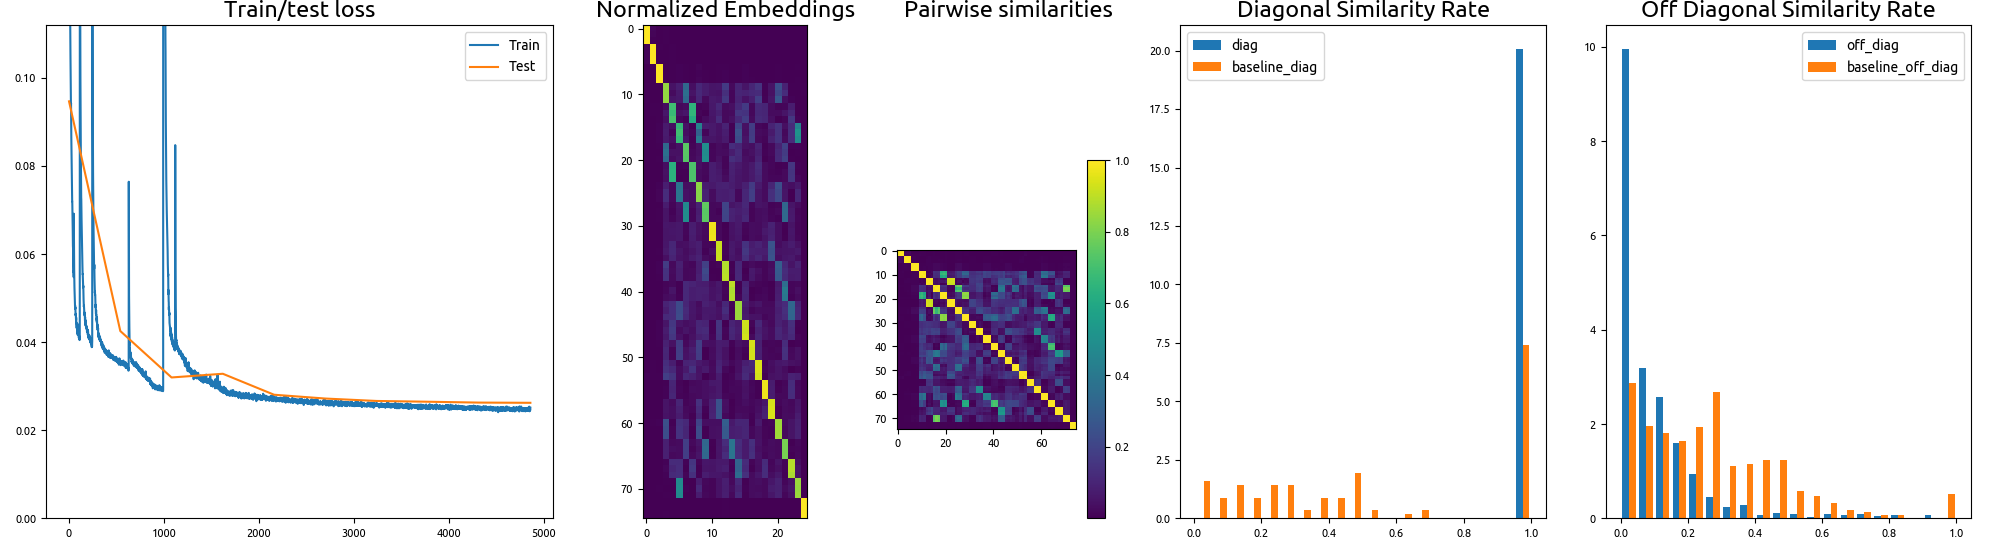
\includegraphics[width=0.9\textwidth]{figures/synth-3view-skip-relu-unsup-false-0}
  \label{fig:synth-3view-skip-relu-unsup-false-0-sub1}
  \caption{Sample embedding, similarity matrix, histogram, and loss curves for best performing of this set}
\end{figure}
\begin{figure}[H]
  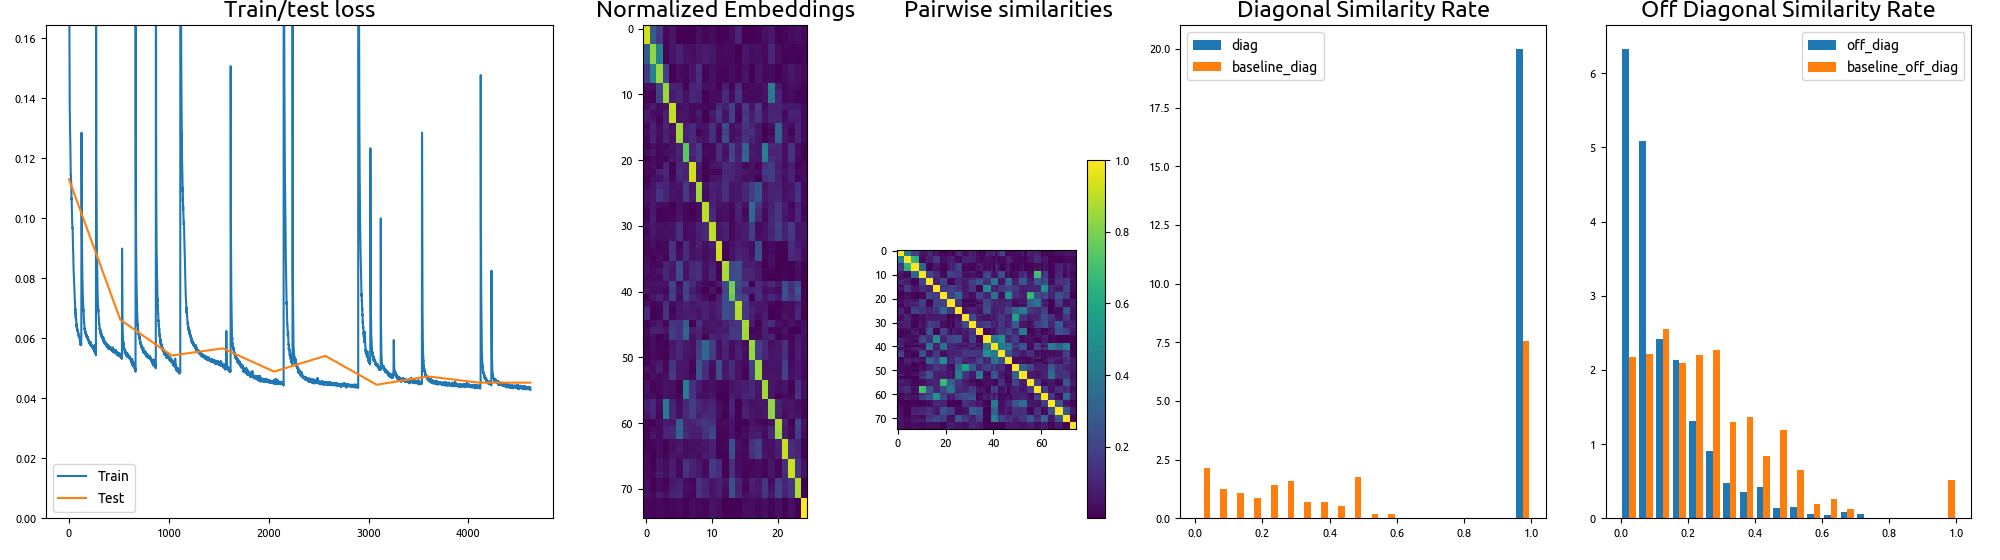
\includegraphics[width=0.9\textwidth]{figures/synth-3view-skip-leakyrelu-unsup-true-0}
  \label{fig:synth-3view-skip-leakyrelu-unsup-true-0-sub1}
  \caption{Sample embedding, similarity matrix, histogram, and loss curves for worst performing of this set}
\end{figure}
\begin{figure}[H]
  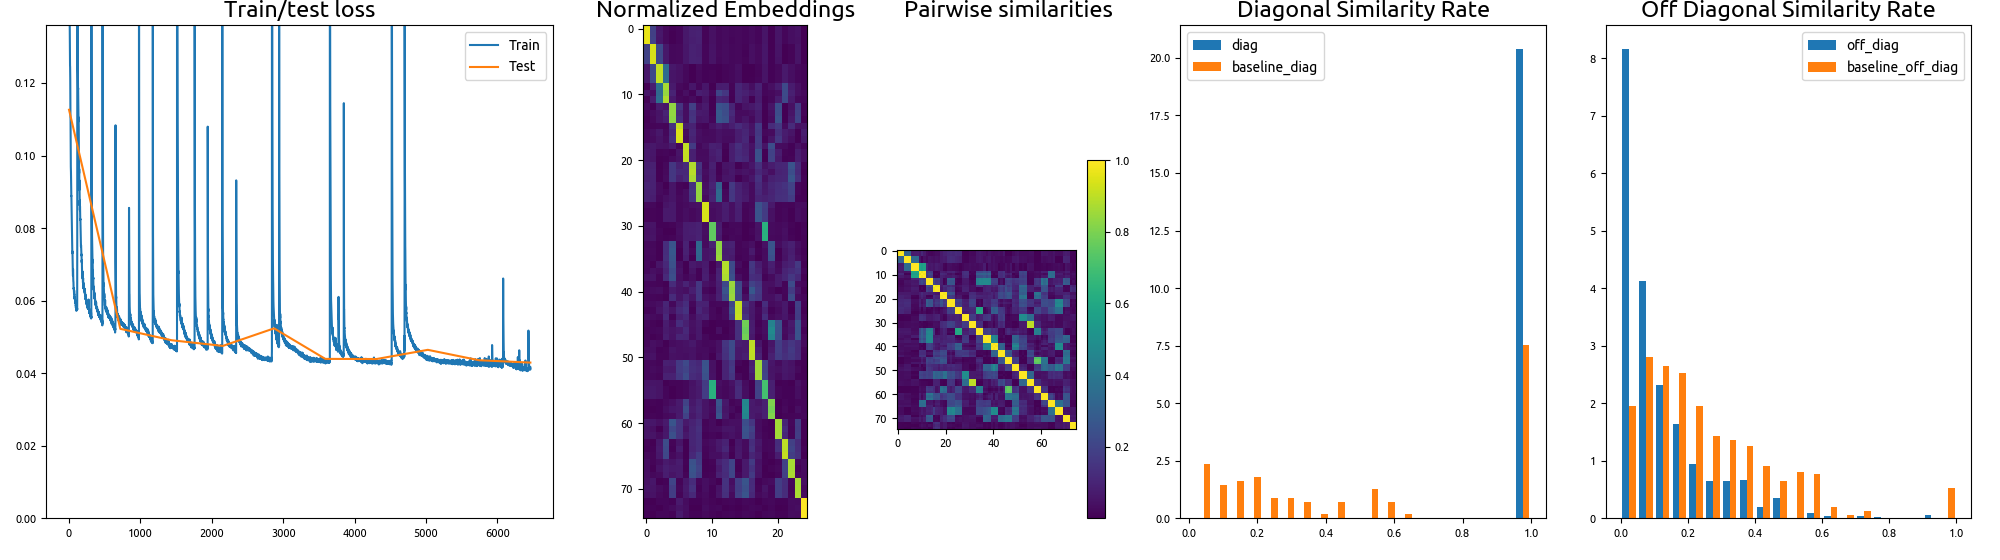
\includegraphics[width=0.9\textwidth]{figures/synth-3view-skip-relu-unsup-true-0}
  \label{fig:synth-3view-skip-relu-unsup-true-0-sub1}
  \caption{Sample embedding, similarity matrix, histogram, and loss curves for random experiment of this set}
\end{figure}
\begin{table}[H]
  \caption{Numerical results}
      \begin{tabular}{|c|c|c|c|} \hline
                                      &  Same Point Similarities  &  Different Point Similarities  \\ \hline
Baseline   & 5.11e-01 $\pm$ 3.90e-01 & 2.56e-01 $\pm$ 2.06e-01 \\ \hline
Skip Type 0 Arch., LeakyReLU, Supervised   & 9.92e-01 $\pm$ 1.68e-02 & 1.10e-01 $\pm$ 1.32e-01 \\ \hline
Skip Type 0 Arch., LeakyReLU, Unsupervised   & 9.97e-01 $\pm$ 6.13e-03 & 1.25e-01 $\pm$ 1.31e-01 \\ \hline
Skip Type 0 Arch., ReLU, Supervised   & 9.98e-01 $\pm$ 4.96e-03 & 9.04e-02 $\pm$ 1.37e-01 \\ \hline
Skip Type 0 Arch., ReLU, Unsupervised   & 9.98e-01 $\pm$ 5.27e-03 & 1.19e-01 $\pm$ 1.30e-01 \\ \hline
Skip Type 1 Arch., LeakyReLU, Supervised   & 9.97e-01 $\pm$ 7.39e-03 & 9.74e-02 $\pm$ 1.38e-01 \\ \hline
Skip Type 1 Arch., LeakyReLU, Unsupervised   & 9.94e-01 $\pm$ 1.04e-02 & 1.21e-01 $\pm$ 1.31e-01 \\ \hline
Skip Type 1 Arch., ReLU, Supervised   & 9.98e-01 $\pm$ 5.89e-03 & 8.48e-02 $\pm$ 1.41e-01 \\ \hline
Skip Type 1 Arch., ReLU, Unsupervised   & 9.96e-01 $\pm$ 7.70e-03 & 1.16e-01 $\pm$ 1.32e-01 \\ \hline
      \end{tabular}
      \label{fig:12_tab1}
\end{table}



\subsubsection*{Experiment Run 13}
Using ReLU activation type with aforementioned pairwise noise. 
The ``Long Skip'' type architecture is basically the skip type but with additional skip connections from layer 1 to layer $n/2$ and layer $n$.
This helps training and performance a fair amount since it allows way more layers (doubling or tripling). 

\begin{figure}[H]
  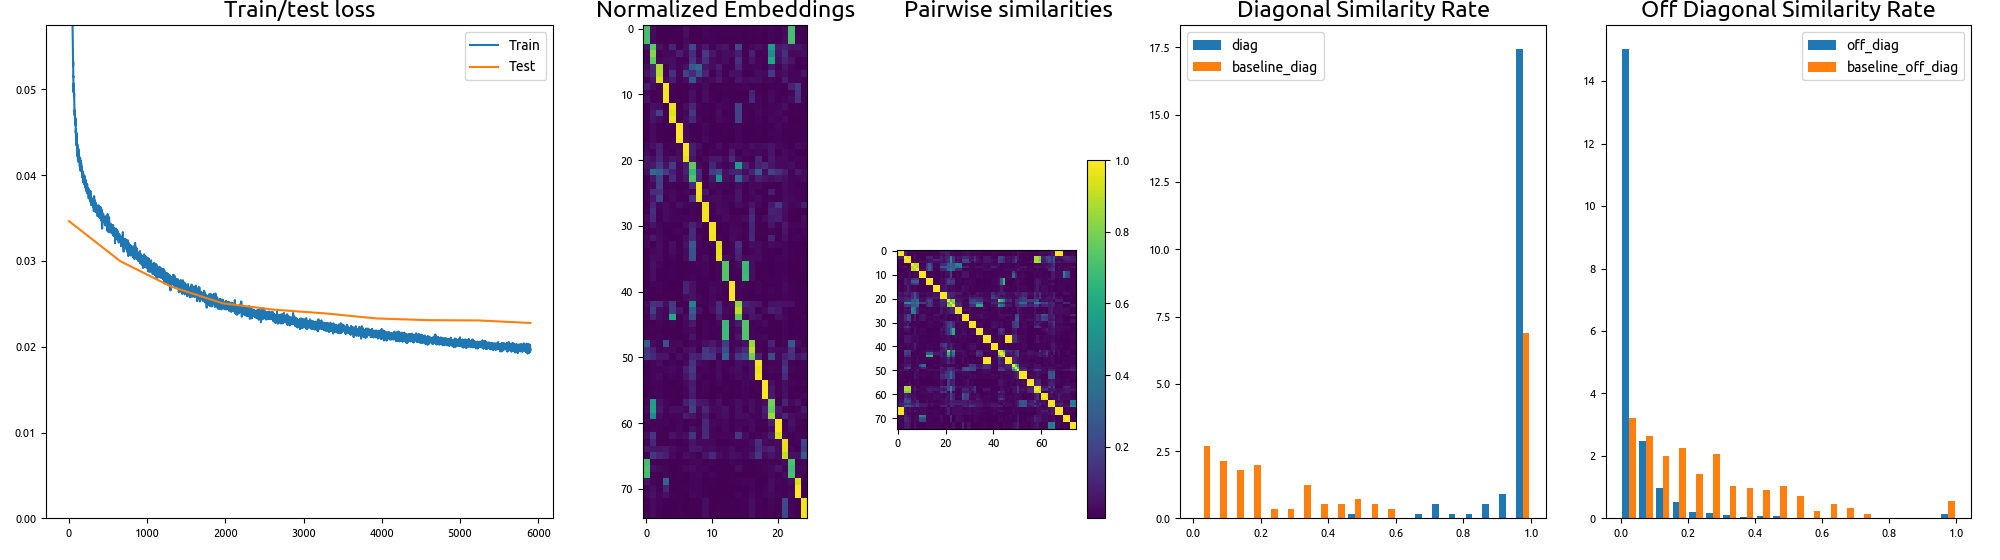
\includegraphics[width=0.9\textwidth]{figures/pairwise5-skip0-relu-ld-false-unsup-true-0}
  \label{fig:pairwise5-skip0-relu-ld-false-unsup-true-0-sub1}
  \caption{Sample embedding, similarity matrix, histogram, and loss curves for best performing of this set}
\end{figure}
\begin{figure}[H]
  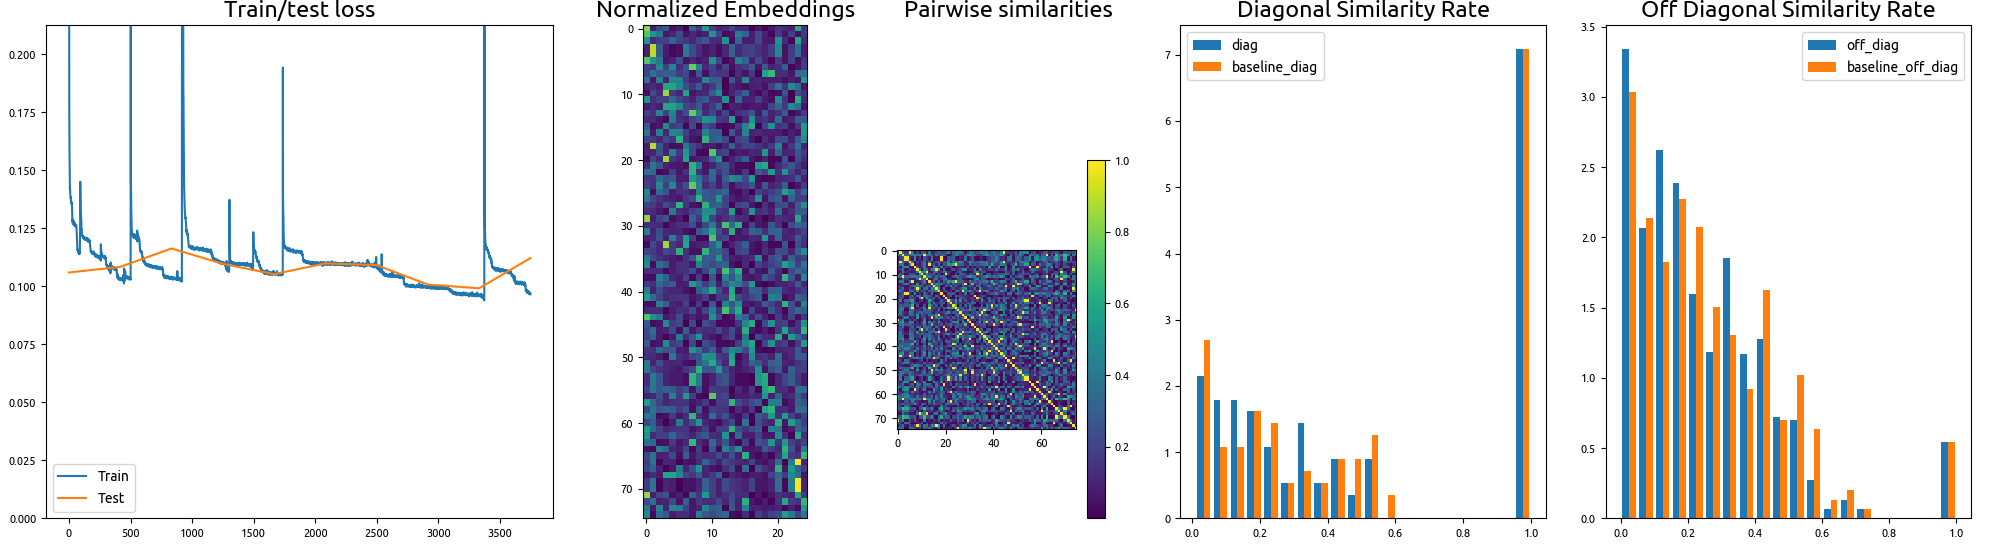
\includegraphics[width=0.9\textwidth]{figures/pairwise3-attn2-relu-ld-true-unsup-false-0}
  \label{fig:pairwise3-attn2-relu-ld-true-unsup-false-0-sub1}
  \caption{Sample embedding, similarity matrix, histogram, and loss curves for worst performing of this set}
\end{figure}
\begin{figure}[H]
  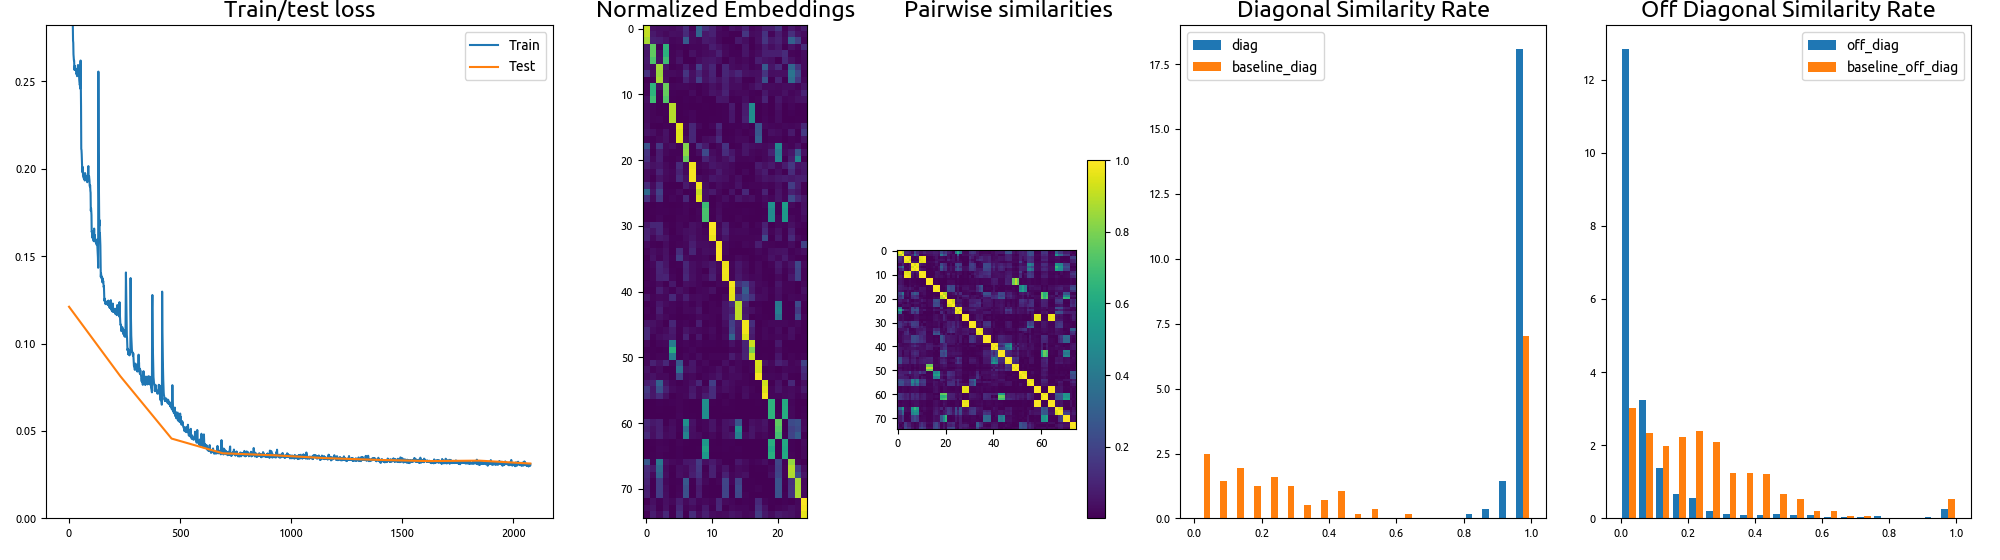
\includegraphics[width=0.9\textwidth]{figures/pairwise3-longskip0-relu-ld-true-unsup-false-0}
  \label{fig:pairwise3-longskip0-relu-ld-true-unsup-false-0-sub1}
  \caption{Sample embedding, similarity matrix, histogram, and loss curves for random experiment of this set}
\end{figure}

\begin{table}[H]
  \caption{\texttt{pairwise3} results}
      \begin{tabular}{|l|c|c|c|} \hline
                                      &  Same Point Similarities  &  Different Point Similarities  \\ \hline
Baseline   & 5.11e-01 $\pm$ 3.90e-01 & 2.56e-01 $\pm$ 2.06e-01 \\ \hline
\multicolumn{3}{|c|}{Data type \texttt{pairwise3} with generated data} \\ \hline
GAT Network Type 0 Arch., Supervised   & 5.75e-01 $\pm$ 3.58e-01 & 2.26e-01 $\pm$ 1.77e-01 \\ \hline
GAT Network Type 0 Arch., Unsupervised   & 7.11e-01 $\pm$ 2.65e-01 & 1.74e-01 $\pm$ 1.41e-01 \\ \hline
GAT Network Type 1 Arch., Supervised   & 5.96e-01 $\pm$ 3.44e-01 & 2.07e-01 $\pm$ 1.65e-01 \\ \hline
GAT Network Type 1 Arch., Unsupervised   & 7.65e-01 $\pm$ 2.36e-01 & 1.87e-01 $\pm$ 1.53e-01 \\ \hline
GAT Network Type 2 Arch., Supervised   & 8.33e-01 $\pm$ 1.79e-01 & 2.17e-01 $\pm$ 1.67e-01 \\ \hline
GAT Network Type 2 Arch., Unsupervised   & 5.13e-01 $\pm$ 3.89e-01 & 1.98e-01 $\pm$ 1.71e-01 \\ \hline
Long Skip Type 0 Arch., Supervised   & 9.90e-01 $\pm$ 2.35e-02 & 7.18e-02 $\pm$ 1.60e-01 \\ \hline
Long Skip Type 0 Arch., Unsupervised   & 9.59e-01 $\pm$ 6.03e-02 & 1.00e-01 $\pm$ 1.57e-01 \\ \hline
Skip Connections Type 1 Arch., Supervised   & 9.74e-01 $\pm$ 5.64e-02 & 9.52e-02 $\pm$ 1.60e-01 \\ \hline
Skip Connections Type 1 Arch., Unsupervised   & 9.66e-01 $\pm$ 7.82e-02 & 8.26e-02 $\pm$ 1.61e-01 \\ \hline
\multicolumn{3}{|c|}{Data type \texttt{pairwise3} with prestored data} \\ \hline
GAT Network Type 0 Arch., Supervised   & 5.95e-01 $\pm$ 3.45e-01 & 2.05e-01 $\pm$ 1.66e-01 \\ \hline
GAT Network Type 0 Arch., Unsupervised   & 6.64e-01 $\pm$ 3.15e-01 & 1.82e-01 $\pm$ 1.68e-01 \\ \hline
GAT Network Type 1 Arch., Supervised   & 5.09e-01 $\pm$ 3.93e-01 & 2.21e-01 $\pm$ 1.87e-01 \\ \hline
GAT Network Type 1 Arch., Unsupervised   & 7.07e-01 $\pm$ 2.76e-01 & 1.64e-01 $\pm$ 1.47e-01 \\ \hline
GAT Network Type 2 Arch., Supervised   & 4.92e-01 $\pm$ 4.00e-01 & 2.30e-01 $\pm$ 1.98e-01 \\ \hline
GAT Network Type 2 Arch., Unsupervised   & 6.12e-01 $\pm$ 3.33e-01 & 2.04e-01 $\pm$ 1.65e-01 \\ \hline
Long Skip Type 0 Arch., Supervised   & 9.80e-01 $\pm$ 3.75e-02 & 8.56e-02 $\pm$ 1.57e-01 \\ \hline
Long Skip Type 0 Arch., Unsupervised   & 9.62e-01 $\pm$ 5.32e-02 & 1.01e-01 $\pm$ 1.61e-01 \\ \hline
Skip Connections Type 1 Arch., Supervised   & 9.73e-01 $\pm$ 6.48e-02 & 8.12e-02 $\pm$ 1.60e-01 \\ \hline
Skip Connections Type 1 Arch., Unsupervised   & 9.66e-01 $\pm$ 7.71e-02 & 8.23e-02 $\pm$ 1.57e-01 \\ \hline
      \end{tabular}
      \label{fig:13_tab1}
\end{table}

\begin{table}[H]
  \caption{\texttt{pairwise5} results}
      \begin{tabular}{|l|c|c|c|} \hline
                                      &  Same Point Similarities  &  Different Point Similarities  \\ \hline
Baseline   & 5.11e-01 $\pm$ 3.90e-01 & 2.56e-01 $\pm$ 2.06e-01 \\ \hline
\multicolumn{3}{|c|}{Data type \texttt{pairwise5} with generated data} \\ \hline
GAT Network Type 0 Arch., Supervised   & 5.04e-01 $\pm$ 3.97e-01 & 2.12e-01 $\pm$ 1.90e-01 \\ \hline
GAT Network Type 0 Arch., Unsupervised   & 7.51e-01 $\pm$ 2.39e-01 & 2.06e-01 $\pm$ 1.57e-01 \\ \hline
GAT Network Type 1 Arch., Supervised   & 6.99e-01 $\pm$ 2.74e-01 & 1.99e-01 $\pm$ 1.53e-01 \\ \hline
GAT Network Type 1 Arch., Unsupervised   & 5.41e-01 $\pm$ 3.74e-01 & 2.16e-01 $\pm$ 1.79e-01 \\ \hline
GAT Network Type 2 Arch., Supervised   & 6.72e-01 $\pm$ 2.90e-01 & 2.01e-01 $\pm$ 1.55e-01 \\ \hline
GAT Network Type 2 Arch., Unsupervised   & 5.09e-01 $\pm$ 3.93e-01 & 1.94e-01 $\pm$ 1.83e-01 \\ \hline
Long Skip Type 0 Arch., Supervised   & 9.68e-01 $\pm$ 5.29e-02 & 9.50e-02 $\pm$ 1.58e-01 \\ \hline
Long Skip Type 0 Arch., Unsupervised   & 9.40e-01 $\pm$ 7.90e-02 & 1.11e-01 $\pm$ 1.54e-01 \\ \hline
Skip Connections Type 1 Arch., Supervised   & 9.69e-01 $\pm$ 7.55e-02 & 6.14e-02 $\pm$ 1.43e-01 \\ \hline
Skip Connections Type 1 Arch., Unsupervised   & 9.66e-01 $\pm$ 8.32e-02 & 6.17e-02 $\pm$ 1.37e-01 \\ \hline
\multicolumn{3}{|c|}{Data type \texttt{pairwise5} with prestored data} \\ \hline
GAT Network Type 0 Arch., Supervised   & 8.06e-01 $\pm$ 2.14e-01 & 1.88e-01 $\pm$ 1.63e-01 \\ \hline
GAT Network Type 0 Arch., Unsupervised   & 5.92e-01 $\pm$ 3.56e-01 & 1.76e-01 $\pm$ 1.71e-01 \\ \hline
GAT Network Type 1 Arch., Supervised   & 4.96e-01 $\pm$ 3.99e-01 & 2.27e-01 $\pm$ 1.97e-01 \\ \hline
GAT Network Type 1 Arch., Unsupervised   & 5.95e-01 $\pm$ 3.44e-01 & 2.06e-01 $\pm$ 1.65e-01 \\ \hline
GAT Network Type 2 Arch., Supervised   & 8.11e-01 $\pm$ 2.06e-01 & 2.02e-01 $\pm$ 1.68e-01 \\ \hline
GAT Network Type 2 Arch., Unsupervised   & 5.84e-01 $\pm$ 3.49e-01 & 1.96e-01 $\pm$ 1.62e-01 \\ \hline
Long Skip Type 0 Arch., Supervised   & 9.66e-01 $\pm$ 5.37e-02 & 9.77e-02 $\pm$ 1.60e-01 \\ \hline
Long Skip Type 0 Arch., Unsupervised   & 9.74e-01 $\pm$ 4.28e-02 & 8.56e-02 $\pm$ 1.51e-01 \\ \hline
Skip Connections Type 1 Arch., Supervised   & 9.69e-01 $\pm$ 7.68e-02 & 6.22e-02 $\pm$ 1.44e-01 \\ \hline
Skip Connections Type 1 Arch., Unsupervised   & 9.65e-01 $\pm$ 8.34e-02 & 6.49e-02 $\pm$ 1.42e-01 \\ \hline
      \end{tabular}
      \label{fig:13_tab2}
\end{table}




\subsubsection*{Experiment Run 14}
Comparison between GAT and Sparse GAT architecture

\begin{figure}[H]
  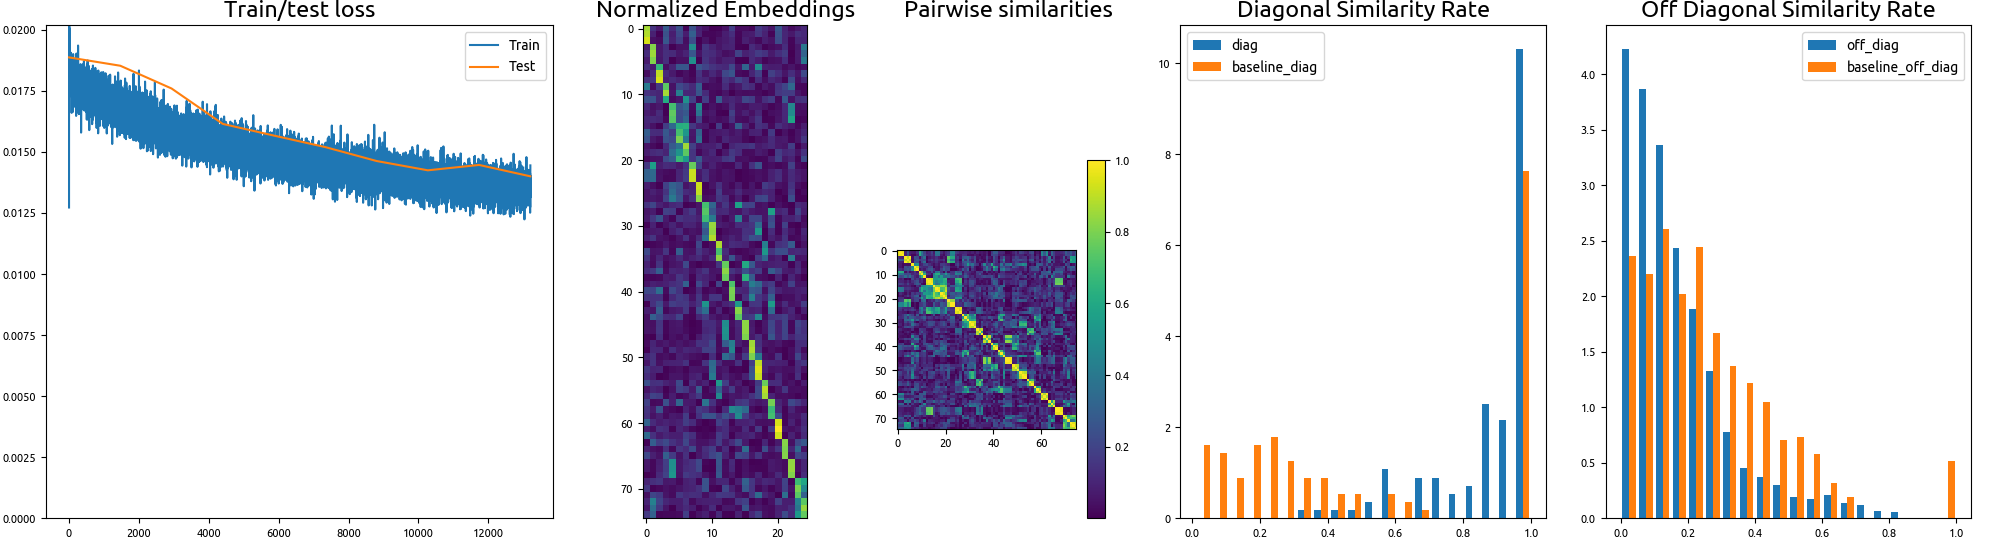
\includegraphics[width=0.9\textwidth]{figures/pairwise3-spattn0-0-0}
  \label{fig:pairwise3-spattn0-0-0-sub1}
  \caption{Sample embedding, similarity matrix, histogram, and loss curves for best performing of this set}
\end{figure}
\begin{figure}[H]
  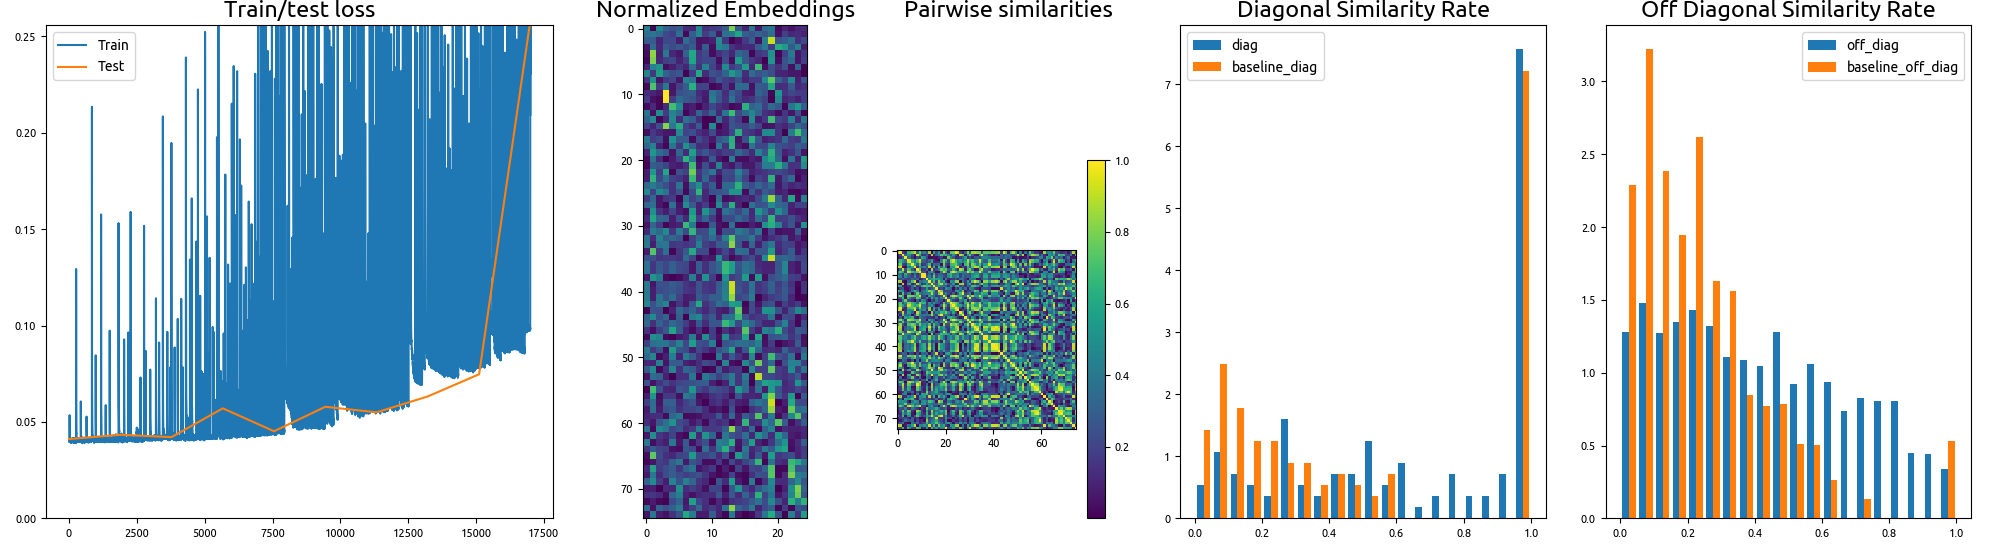
\includegraphics[width=0.9\textwidth]{figures/pairwise5-attn0-0-0}
  \label{fig:pairwise5-attn0-0-0-sub1}
  \caption{Sample embedding, similarity matrix, histogram, and loss curves for worst performing of this set}
\end{figure}
\begin{figure}[H]
  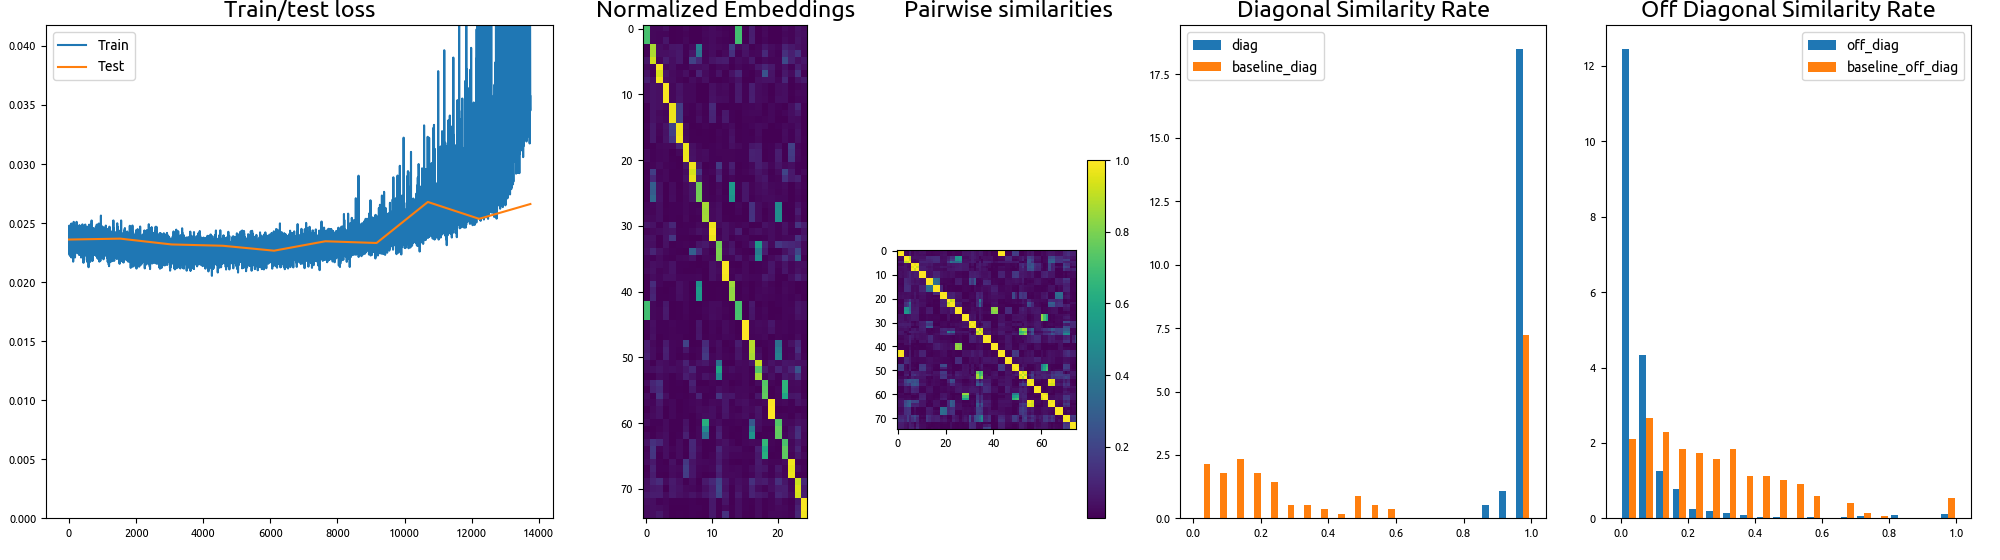
\includegraphics[width=0.9\textwidth]{figures/pairwise3-spattn1-0-1}
  \label{fig:pairwise3-spattn1-0-1-sub1}
  \caption{Sample embedding, similarity matrix, histogram, and loss curves for random experiment of this se}
\end{figure}
\begin{table}[H]
  \caption{Numerical results}
      \begin{tabular}{|c|c|c|c|} \hline
                                      &  Same Point Similarities  &  Different Point Similarities  \\ \hline
Baseline   & 5.12e-01 $\pm$ 3.91e-01 & 2.56e-01 $\pm$ 2.06e-01 \\ \hline
\multicolumn{3}{|c|}{Data type \texttt{pairwise3} with prestored data} \\ \hline
GAT Network Type 0 Architecture   & 7.38e-01 $\pm$ 2.60e-01 & 1.52e-01 $\pm$ 1.55e-01 \\ \hline
GAT Network Type 0 Architecture   & 7.38e-01 $\pm$ 2.60e-01 & 1.52e-01 $\pm$ 1.55e-01 \\ \hline
GAT Network Type 1 Architecture   & 7.19e-01 $\pm$ 2.62e-01 & 1.87e-01 $\pm$ 1.64e-01 \\ \hline
GAT Network Type 1 Architecture   & 7.19e-01 $\pm$ 2.62e-01 & 1.87e-01 $\pm$ 1.64e-01 \\ \hline
Sparse GAT Network Type 0 Architecture   & 8.90e-01 $\pm$ 1.36e-01 & 1.68e-01 $\pm$ 1.61e-01 \\ \hline
Sparse GAT Network Type 0 Architecture   & 8.90e-01 $\pm$ 1.36e-01 & 1.68e-01 $\pm$ 1.61e-01 \\ \hline
Sparse GAT Network Type 1 Architecture   & 9.80e-01 $\pm$ 5.07e-02 & 8.68e-02 $\pm$ 1.43e-01 \\ \hline
Sparse GAT Network Type 1 Architecture   & 9.80e-01 $\pm$ 5.07e-02 & 8.68e-02 $\pm$ 1.43e-01 \\ \hline
\multicolumn{3}{|c|}{Data type \texttt{pairwise5} with prestored data} \\ \hline
GAT Network Type 0 Architecture   & 6.83e-01 $\pm$ 3.22e-01 & 4.33e-01 $\pm$ 2.63e-01 \\ \hline
GAT Network Type 0 Architecture   & 6.83e-01 $\pm$ 3.22e-01 & 4.33e-01 $\pm$ 2.63e-01 \\ \hline
GAT Network Type 1 Architecture   & 6.36e-01 $\pm$ 3.54e-01 & 1.97e-01 $\pm$ 2.00e-01 \\ \hline
GAT Network Type 1 Architecture   & 6.36e-01 $\pm$ 3.54e-01 & 1.97e-01 $\pm$ 2.00e-01 \\ \hline
Sparse GAT Network Type 0 Architecture   & 9.50e-01 $\pm$ 8.77e-02 & 1.16e-01 $\pm$ 1.49e-01 \\ \hline
Sparse GAT Network Type 0 Architecture   & 9.50e-01 $\pm$ 8.77e-02 & 1.16e-01 $\pm$ 1.49e-01 \\ \hline
Sparse GAT Network Type 1 Architecture   & 6.24e-01 $\pm$ 3.50e-01 & 3.99e-01 $\pm$ 2.62e-01 \\ \hline
Sparse GAT Network Type 1 Architecture   & 6.24e-01 $\pm$ 3.50e-01 & 3.99e-01 $\pm$ 2.62e-01 \\ \hline
\multicolumn{3}{|c|}{Data type \texttt{pairwise5} with data generation} \\ \hline
GAT Network Type 0 Architecture   & 5.26e-01 $\pm$ 3.87e-01 & 2.31e-01 $\pm$ 1.94e-01 \\ \hline
GAT Network Type 0 Architecture   & 5.26e-01 $\pm$ 3.87e-01 & 2.31e-01 $\pm$ 1.94e-01 \\ \hline
GAT Network Type 0 Architecture   & 4.87e-01 $\pm$ 4.07e-01 & 2.13e-01 $\pm$ 2.00e-01 \\ \hline
GAT Network Type 0 Architecture   & 4.87e-01 $\pm$ 4.07e-01 & 2.13e-01 $\pm$ 2.00e-01 \\ \hline
GAT Network Type 0 Architecture   & 4.88e-01 $\pm$ 4.06e-01 & 2.17e-01 $\pm$ 1.97e-01 \\ \hline
GAT Network Type 0 Architecture   & 4.88e-01 $\pm$ 4.06e-01 & 2.17e-01 $\pm$ 1.97e-01 \\ \hline
GAT Network Type 0 Architecture   & 4.87e-01 $\pm$ 4.02e-01 & 2.23e-01 $\pm$ 1.98e-01 \\ \hline
GAT Network Type 0 Architecture   & 4.87e-01 $\pm$ 4.02e-01 & 2.23e-01 $\pm$ 1.98e-01 \\ \hline
Sparse GAT Network Type 0 Architecture   & 9.30e-01 $\pm$ 1.36e-01 & 1.42e-01 $\pm$ 1.53e-01 \\ \hline
Sparse GAT Network Type 0 Architecture   & 9.30e-01 $\pm$ 1.36e-01 & 1.42e-01 $\pm$ 1.53e-01 \\ \hline
Sparse GAT Network Type 0 Architecture   & 9.31e-01 $\pm$ 1.23e-01 & 1.33e-01 $\pm$ 1.56e-01 \\ \hline
Sparse GAT Network Type 0 Architecture   & 9.31e-01 $\pm$ 1.23e-01 & 1.33e-01 $\pm$ 1.56e-01 \\ \hline
Sparse GAT Network Type 0 Architecture   & 8.81e-01 $\pm$ 1.57e-01 & 1.51e-01 $\pm$ 1.48e-01 \\ \hline
Sparse GAT Network Type 0 Architecture   & 8.81e-01 $\pm$ 1.57e-01 & 1.51e-01 $\pm$ 1.48e-01 \\ \hline
Sparse GAT Network Type 0 Architecture   & 9.30e-01 $\pm$ 1.17e-01 & 1.38e-01 $\pm$ 1.57e-01 \\ \hline
Sparse GAT Network Type 0 Architecture   & 9.30e-01 $\pm$ 1.17e-01 & 1.38e-01 $\pm$ 1.57e-01 \\ \hline
      \end{tabular}
      \label{fig:{0}_tab1}
\end{table}

\subsubsection*{Experiment Run 16}
(Run 16 had some errors)
Testing on outliers. An outlier is the following noise model:
\begin{equation*}
Hi
\end{equation*}
All the architectures are of type Long Skip Type 0 Arch. (\texttt{longskip0}).

\begin{figure}[H]
  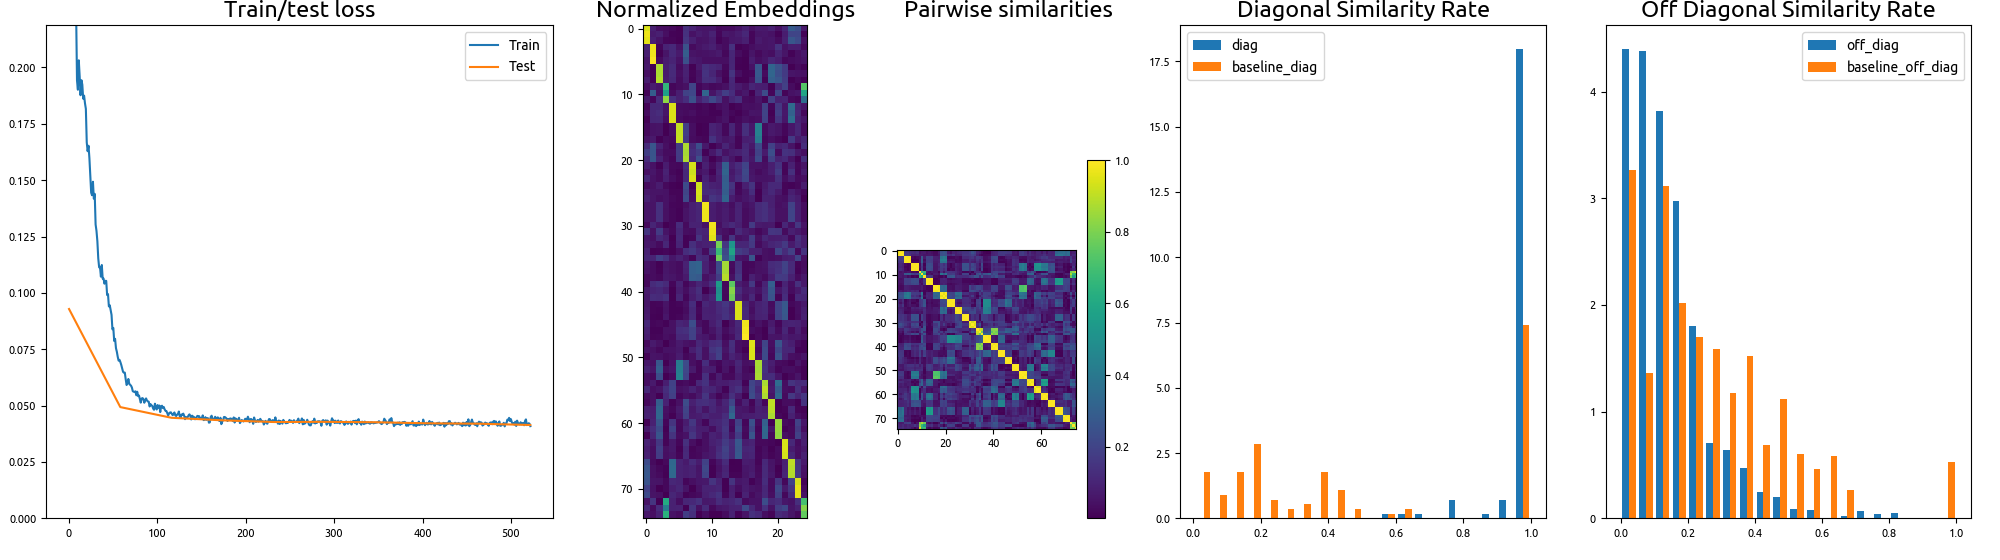
\includegraphics[width=0.9\textwidth]{figures/outlier1-longskip0-load-false-1}
  \label{fig:outlier1-longskip0-load-false-1-sub1}
  \caption{Sample embedding, similarity matrix, histogram, and loss curves for best performing of this set}
\end{figure}
\begin{figure}[H]
  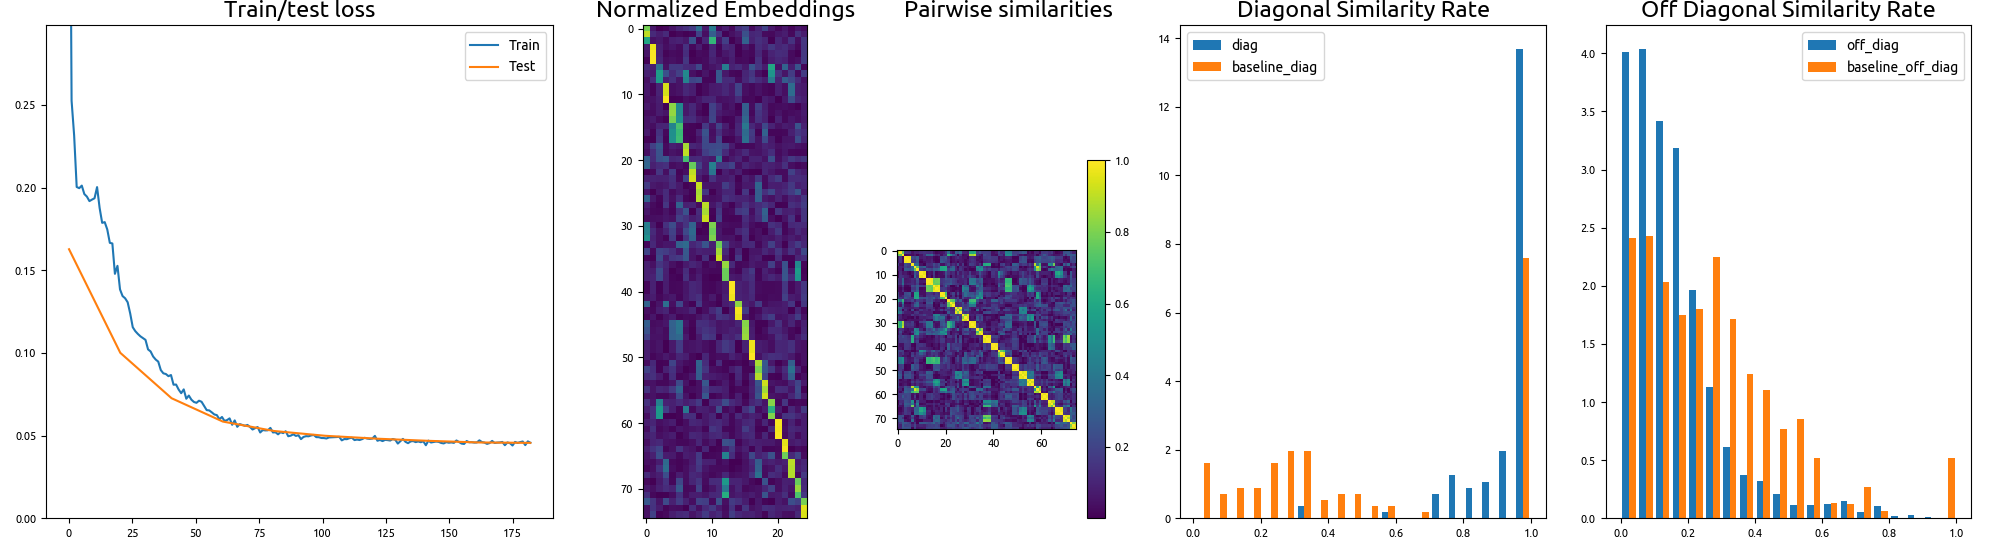
\includegraphics[width=0.9\textwidth]{figures/outlier8-longskip0-load-false-0}
  \label{fig:outlier8-longskip0-load-false-0-sub1}
  \caption{Sample embedding, similarity matrix, histogram, and loss curves for worst performing of this set}
\end{figure}
\begin{figure}[H]
  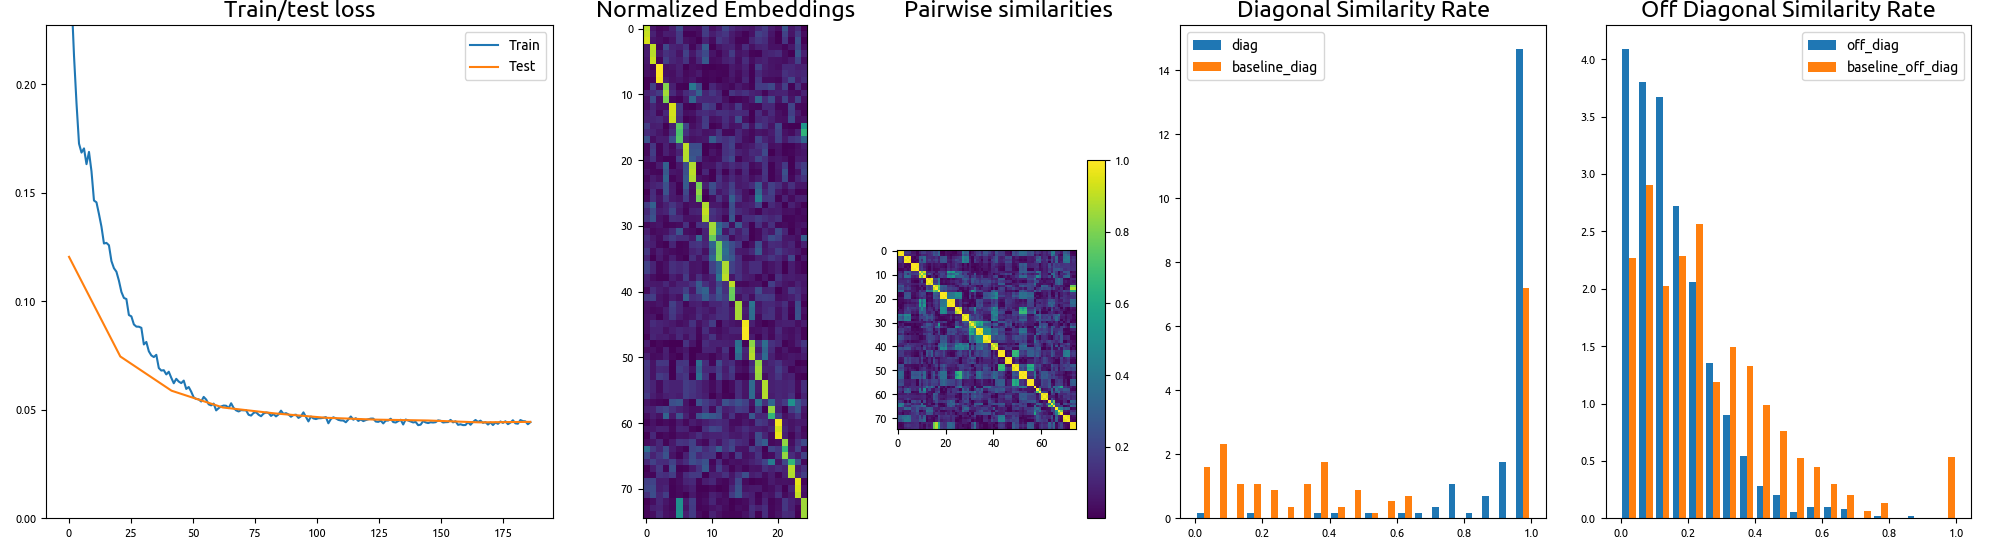
\includegraphics[width=0.9\textwidth]{figures/outlier2-longskip0-load-false-1}
  \label{fig:outlier2-longskip0-load-false-1-sub1}
  \caption{Sample embedding, similarity matrix, histogram, and loss curves for random experiment of this set}
\end{figure}

\begin{table}[H]
  \caption{Numerical results}
      \begin{tabular}{|l|c|c|c|} \hline
                                      &  Same Point Similarities  &  Different Point Similarities  \\ \hline
Baseline   & 5.10e-01 $\pm$ 3.90e-01 & 2.56e-01 $\pm$ 2.06e-01 \\ \hline
Data type \texttt{outlier1} & 9.73e-01 $\pm$ 9.43e-02 & 1.53e-01 $\pm$ 1.39e-01 \\ \hline
Data type \texttt{outlier1} & 9.75e-01 $\pm$ 7.25e-02 & 1.51e-01 $\pm$ 1.44e-01 \\ \hline
Data type \texttt{outlier1} & 9.70e-01 $\pm$ 9.98e-02 & 1.53e-01 $\pm$ 1.40e-01 \\ \hline
Data type \texttt{outlier2} & 9.28e-01 $\pm$ 1.51e-01 & 1.57e-01 $\pm$ 1.39e-01 \\ \hline
Data type \texttt{outlier2} & 9.38e-01 $\pm$ 1.43e-01 & 1.60e-01 $\pm$ 1.38e-01 \\ \hline
Data type \texttt{outlier2} & 9.46e-01 $\pm$ 1.32e-01 & 1.50e-01 $\pm$ 1.36e-01 \\ \hline
Data type \texttt{outlier4} & 9.33e-01 $\pm$ 1.79e-01 & 1.46e-01 $\pm$ 1.50e-01 \\ \hline
Data type \texttt{outlier4} & 9.17e-01 $\pm$ 1.74e-01 & 1.58e-01 $\pm$ 1.41e-01 \\ \hline
Data type \texttt{outlier4} & 9.29e-01 $\pm$ 1.79e-01 & 1.41e-01 $\pm$ 1.48e-01 \\ \hline
Data type \texttt{outlier8} & 8.99e-01 $\pm$ 1.95e-01 & 1.61e-01 $\pm$ 1.40e-01 \\ \hline
Data type \texttt{outlier8} & 9.27e-01 $\pm$ 1.79e-01 & 1.40e-01 $\pm$ 1.51e-01 \\ \hline
Data type \texttt{outlier8} & 9.22e-01 $\pm$ 1.97e-01 & 1.35e-01 $\pm$ 1.53e-01 \\ \hline
      \end{tabular}
      \label{fig:tab1}
\end{table}

\subsubsection*{Experiment Run 17}
This was experimenting to see if we could handle more views. As the Long Skip type architectures seemed to work better. 

\begin{figure}[H]
  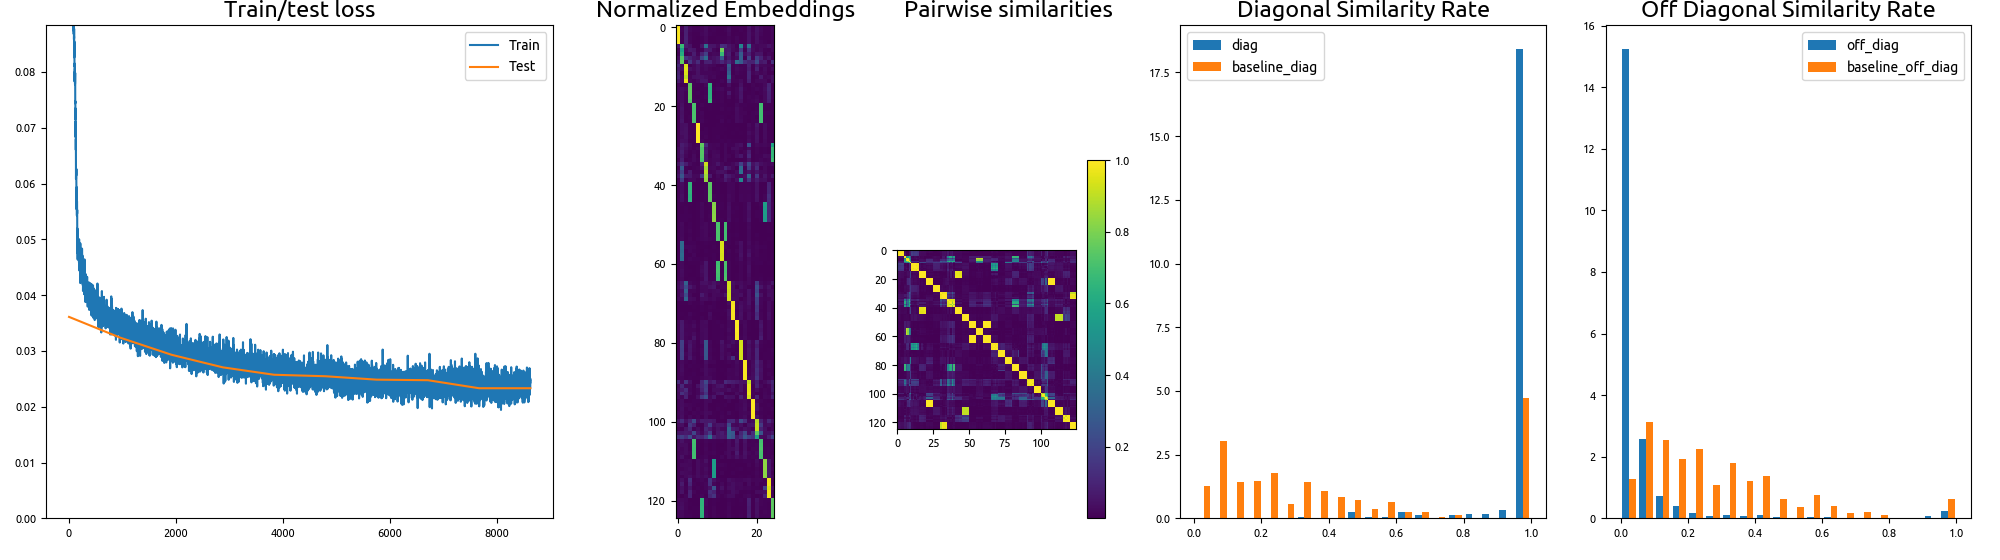
\includegraphics[width=0.9\textwidth]{figures/pairwise5view5-longskip0-load-true-1}
  \label{fig:pairwise5view5-longskip0-load-true-1-sub1}
  \caption{Sample embedding, similarity matrix, histogram, and loss curves for best performing of this set}
\end{figure}
\begin{figure}[H]
  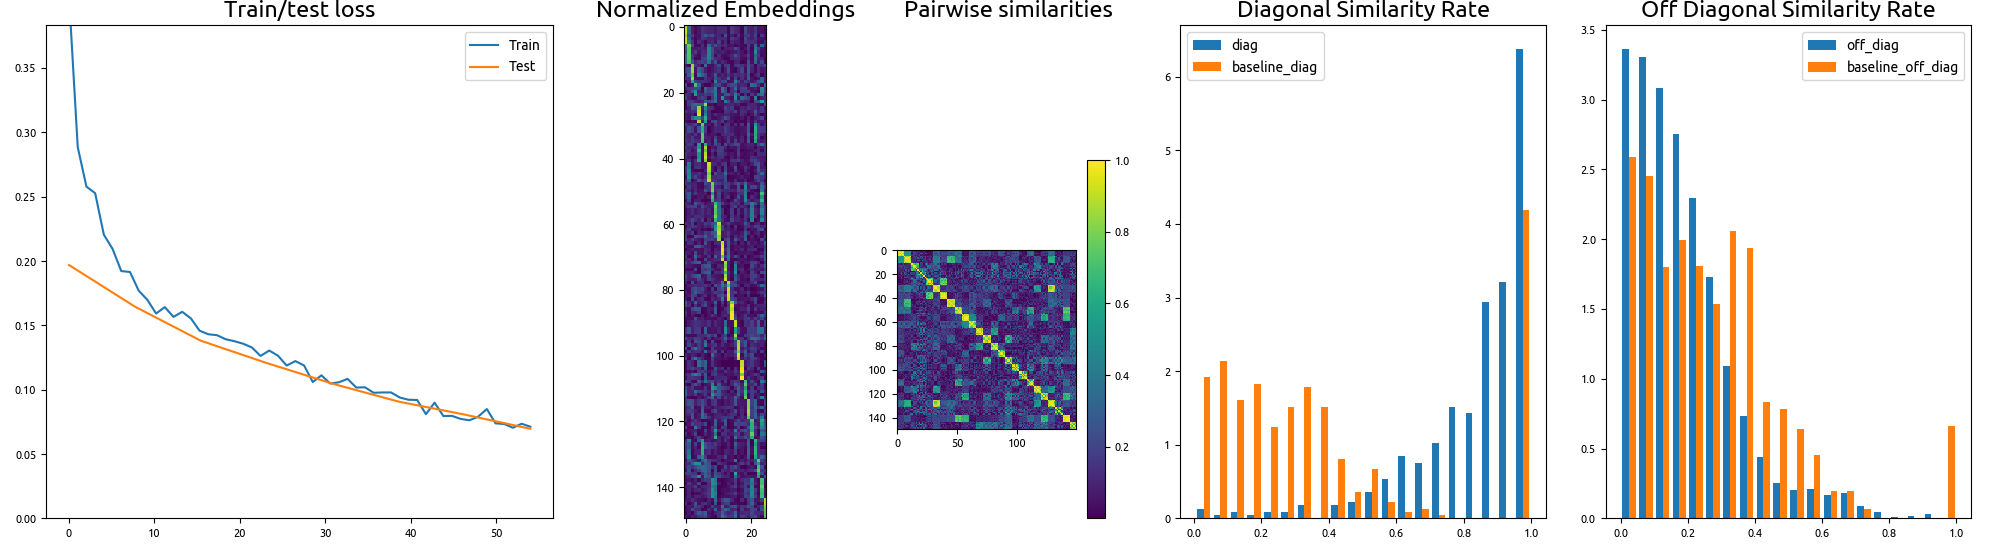
\includegraphics[width=0.9\textwidth]{figures/6view-longskip0-load-true-0}
  \label{fig:6view-longskip0-load-true-0-sub1}
  \caption{Sample embedding, similarity matrix, histogram, and loss curves for worst performing of this set}
\end{figure}
\begin{figure}[H]
  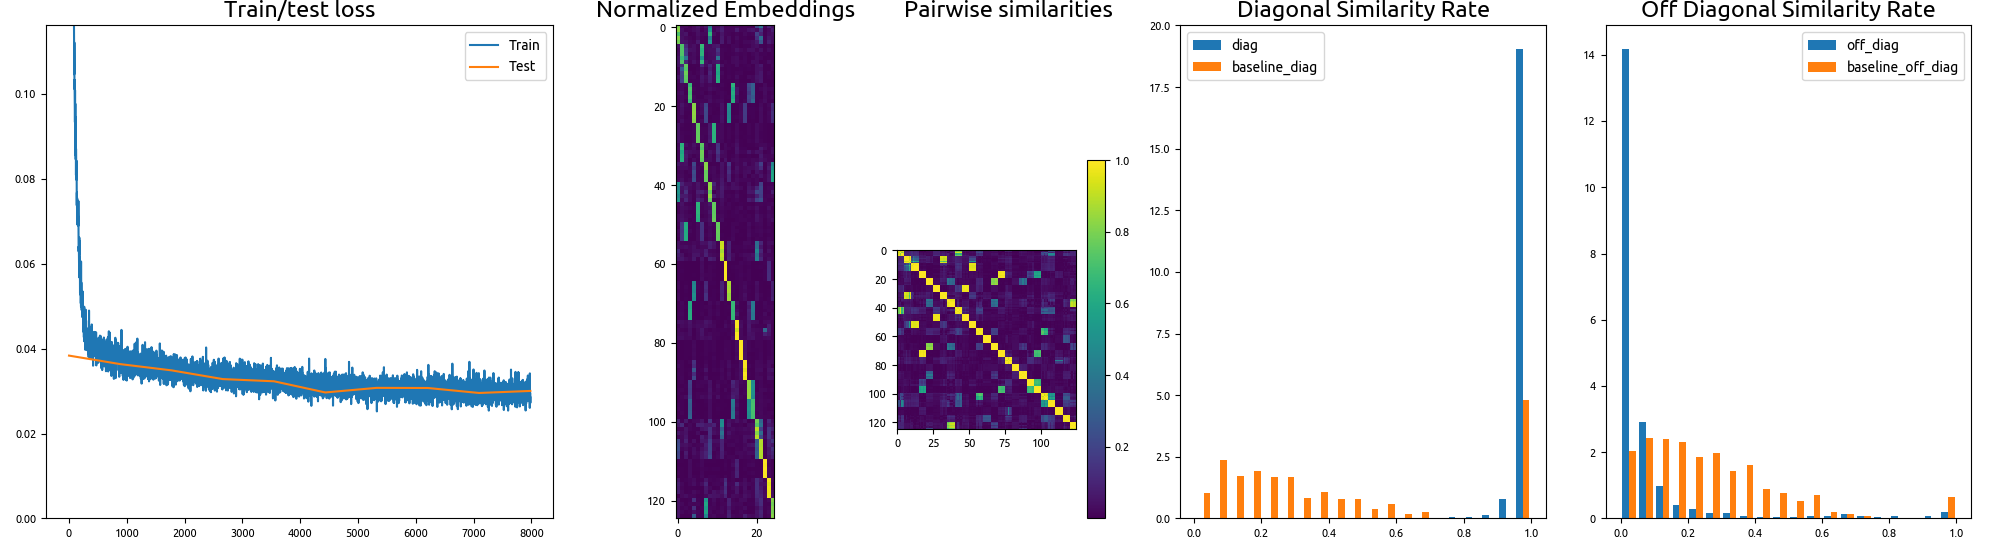
\includegraphics[width=0.9\textwidth]{figures/pairwise3view5-longskip1-load-true-1}
  \label{fig:pairwise3view5-longskip1-load-true-1-sub1}
  \caption{Sample embedding, similarity matrix, histogram, and loss curves for random experiment of this set}
\end{figure}

\begin{table}[H]
  \caption{Numerical results}
      \begin{tabular}{|l|c|c|c|} \hline
                                      &  Same Point Similarities  &  Different Point Similarities  \\ \hline
Baseline   & 4.14e-01 $\pm$ 3.54e-01 & 2.61e-01 $\pm$ 2.13e-01 \\ \hline
\multicolumn{3}{|c|}{Data type \texttt{4view} with prestored data} \\ \hline
Long Skip Type 0 Arch.   & 9.47e-01 $\pm$ 8.19e-02 & 1.61e-01 $\pm$ 1.41e-01 \\ \hline
Long Skip Type 0 Arch.   & 1.00e+00 $\pm$ 1.14e-03 & 1.53e-01 $\pm$ 1.37e-01 \\ \hline
Long Skip Type 0 Arch.   & 9.06e-01 $\pm$ 1.32e-01 & 1.59e-01 $\pm$ 1.53e-01 \\ \hline
Long Skip Type 1 Arch.   & 1.00e+00 $\pm$ 2.75e-04 & 1.24e-01 $\pm$ 1.72e-01 \\ \hline
Long Skip Type 1 Arch.   & 1.00e+00 $\pm$ 6.56e-04 & 1.17e-01 $\pm$ 1.72e-01 \\ \hline
Long Skip Type 1 Arch.   & 9.99e-01 $\pm$ 4.87e-03 & 1.51e-01 $\pm$ 1.38e-01 \\ \hline
\multicolumn{3}{|c|}{Data type \texttt{5view} with prestored data} \\ \hline
Long Skip Type 0 Arch.   & 8.96e-01 $\pm$ 1.33e-01 & 1.66e-01 $\pm$ 1.62e-01 \\ \hline
Long Skip Type 0 Arch.   & 9.99e-01 $\pm$ 2.73e-03 & 1.50e-01 $\pm$ 1.37e-01 \\ \hline
Long Skip Type 0 Arch.   & 1.00e+00 $\pm$ 1.30e-03 & 1.50e-01 $\pm$ 1.35e-01 \\ \hline
Long Skip Type 1 Arch.   & 1.00e+00 $\pm$ 4.15e-04 & 1.22e-01 $\pm$ 1.67e-01 \\ \hline
Long Skip Type 1 Arch.   & 9.99e-01 $\pm$ 2.63e-03 & 1.52e-01 $\pm$ 1.44e-01 \\ \hline
Long Skip Type 1 Arch.   & 9.99e-01 $\pm$ 2.98e-03 & 1.50e-01 $\pm$ 1.43e-01 \\ \hline
\multicolumn{3}{|c|}{Data type \texttt{6view} with prestored data} \\ \hline
Long Skip Type 0 Arch.   & 8.48e-01 $\pm$ 1.75e-01 & 1.98e-01 $\pm$ 1.72e-01 \\ \hline
Long Skip Type 0 Arch.   & 9.98e-01 $\pm$ 5.64e-03 & 1.48e-01 $\pm$ 1.42e-01 \\ \hline
Long Skip Type 0 Arch.   & 9.99e-01 $\pm$ 3.27e-03 & 1.50e-01 $\pm$ 1.36e-01 \\ \hline
Long Skip Type 1 Arch.   & 9.99e-01 $\pm$ 1.93e-03 & 1.47e-01 $\pm$ 1.39e-01 \\ \hline
Long Skip Type 1 Arch.   & 1.00e+00 $\pm$ 6.77e-04 & 1.26e-01 $\pm$ 1.82e-01 \\ \hline
Long Skip Type 1 Arch.   & 1.00e+00 $\pm$ 1.76e-03 & 1.24e-01 $\pm$ 1.75e-01 \\ \hline
\multicolumn{3}{|c|}{Data type \texttt{pairwise3view5} with prestored data} \\ \hline
Long Skip Type 0 Arch.   & 9.86e-01 $\pm$ 2.63e-02 & 9.36e-02 $\pm$ 1.57e-01 \\ \hline
Long Skip Type 0 Arch.   & 9.79e-01 $\pm$ 3.44e-02 & 1.06e-01 $\pm$ 1.64e-01 \\ \hline
Long Skip Type 1 Arch.   & 9.80e-01 $\pm$ 2.63e-02 & 1.14e-01 $\pm$ 1.60e-01 \\ \hline
Long Skip Type 1 Arch.   & 9.89e-01 $\pm$ 2.47e-02 & 7.67e-02 $\pm$ 1.56e-01 \\ \hline
\multicolumn{3}{|c|}{Data type \texttt{pairwise3view6} with prestored data} \\ \hline
Long Skip Type 0 Arch.   & 8.98e-01 $\pm$ 9.67e-02 & 1.51e-01 $\pm$ 1.51e-01 \\ \hline
Long Skip Type 0 Arch.   & 9.84e-01 $\pm$ 3.16e-02 & 7.46e-02 $\pm$ 1.57e-01 \\ \hline
Long Skip Type 1 Arch.   & 8.37e-01 $\pm$ 1.51e-01 & 1.47e-01 $\pm$ 1.61e-01 \\ \hline
Long Skip Type 1 Arch.   & 8.39e-01 $\pm$ 1.63e-01 & 1.37e-01 $\pm$ 1.51e-01 \\ \hline
\multicolumn{3}{|c|}{Data type \texttt{pairwise5view5} with prestored data} \\ \hline
Long Skip Type 0 Arch.   & 9.65e-01 $\pm$ 5.54e-02 & 1.07e-01 $\pm$ 1.57e-01 \\ \hline
Long Skip Type 0 Arch.   & 9.86e-01 $\pm$ 4.68e-02 & 5.57e-02 $\pm$ 1.38e-01 \\ \hline
Long Skip Type 1 Arch.   & 9.68e-01 $\pm$ 4.40e-02 & 1.20e-01 $\pm$ 1.47e-01 \\ \hline
Long Skip Type 1 Arch.   & 9.90e-01 $\pm$ 2.68e-02 & 5.84e-02 $\pm$ 1.37e-01 \\ \hline
      \end{tabular}
      \label{fig:tab1}
\end{table}



\subsubsection*{Thoughts}
To my dismay, the GAT architecture seems very unstable to train and doesn't converge very well if at all. Comparitavely, the best results come from stacking many layers - on the order of 15 seems to work for these problems pretty well. Now the best thing to do would be to go to real data since these seem to be working pretty well. To get better results we really do need additional losses though.
On the flip side, the Long Skip was a great discovery and works really well, much better than any of the previous architectures. It needs to get more layers for more views... this I am guessing a fundamental limitation. I wonder if there is a way to get around this.


\entry{2018}{10}{08}
\subsubsection*{Rome16K dataset}
Formatting this dataset took much longer than expected but I managed to build a parser for it, and now can generate data. The dataset is quite large - I had to subsample it, but if I used the whole thing there would be 1 million examples of triplets

\subsubsection*{Rome16K Experiments Round 1}
These initial experiments were a failure, so I did some experimentation with the learning rate afterward

\begin{figure}[H]
  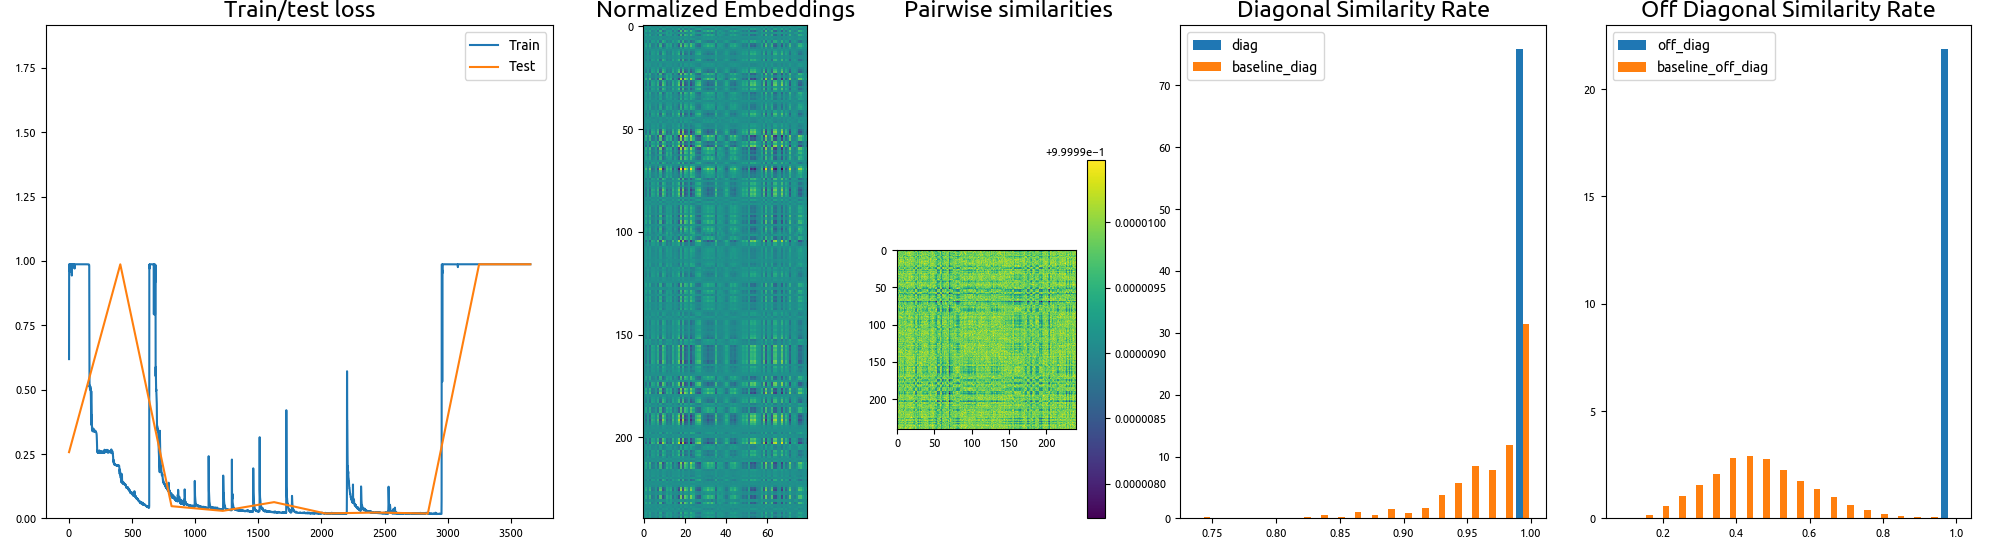
\includegraphics[width=0.9\textwidth]{figures/rome16kknn0-longskip0-load-true-0}
  \label{fig:rome16kknn0-longskip0-load-true-0-sub1}
  \caption{Sample embedding, similarity matrix, histogram, and loss curves for best performing of this set}
\end{figure}
\begin{figure}[H]
  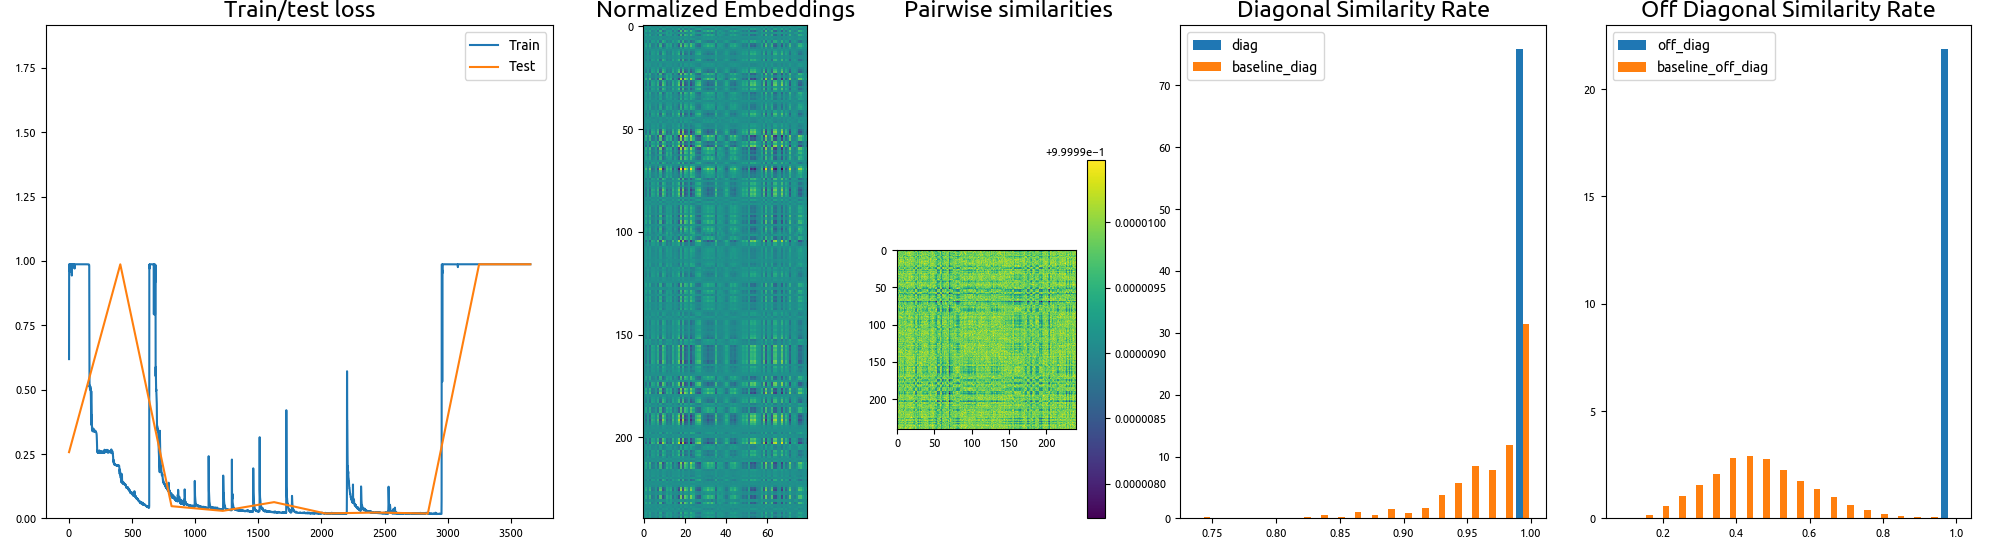
\includegraphics[width=0.9\textwidth]{figures/rome16kknn0-longskip0-load-true-0}
  \label{fig:rome16kknn0-longskip0-load-true-0-sub1}
  \caption{Sample embedding, similarity matrix, histogram, and loss curves for worst performing of this set}
\end{figure}
\begin{table}[H]
  \caption{Numerical results}
      \begin{tabular}{|l|c|c|c|} \hline
                                      &  Same Point Similarities  &  Different Point Similarities  \\ \hline
Baseline   & 9.71e-01 $\pm$ 3.87e-02 & 4.75e-01 $\pm$ 1.42e-01 \\ \hline
Long Skip Type 0 Architecture   & 1.00e+00 $\pm$ 1.64e-07 & 1.00e+00 $\pm$ 3.28e-07 \\ \hline
Long Skip Type 1 Architecture   & 1.00e+00 $\pm$ 1.66e-06 & 1.00e+00 $\pm$ 1.37e-06 \\ \hline
      \end{tabular}
      \label{fig:tab1}
\end{table}

\subsubsection*{Rome16K Experiments Round 2}
This seem to work better - using a learning rate of 1e-4 seemed to work best

\begin{figure}[H]
  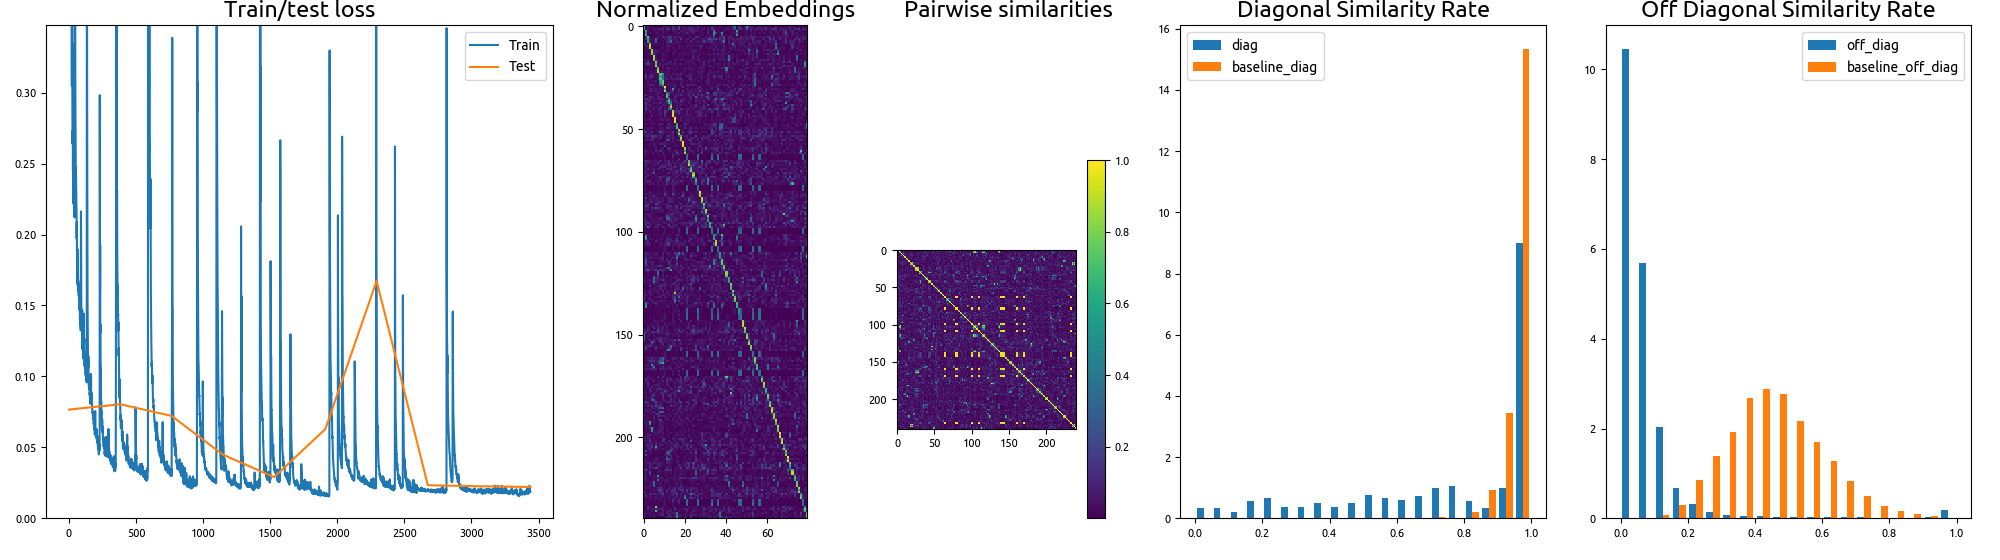
\includegraphics[width=0.9\textwidth]{figures/rome16kknn0-longskip0-lr-1e-4-0}
  \label{fig:rome16kknn0-longskip0-lr-1e-4-0-sub1}
  \caption{Sample embedding, similarity matrix, histogram, and loss curves for best performing of this set}
\end{figure}
\begin{figure}[H]
  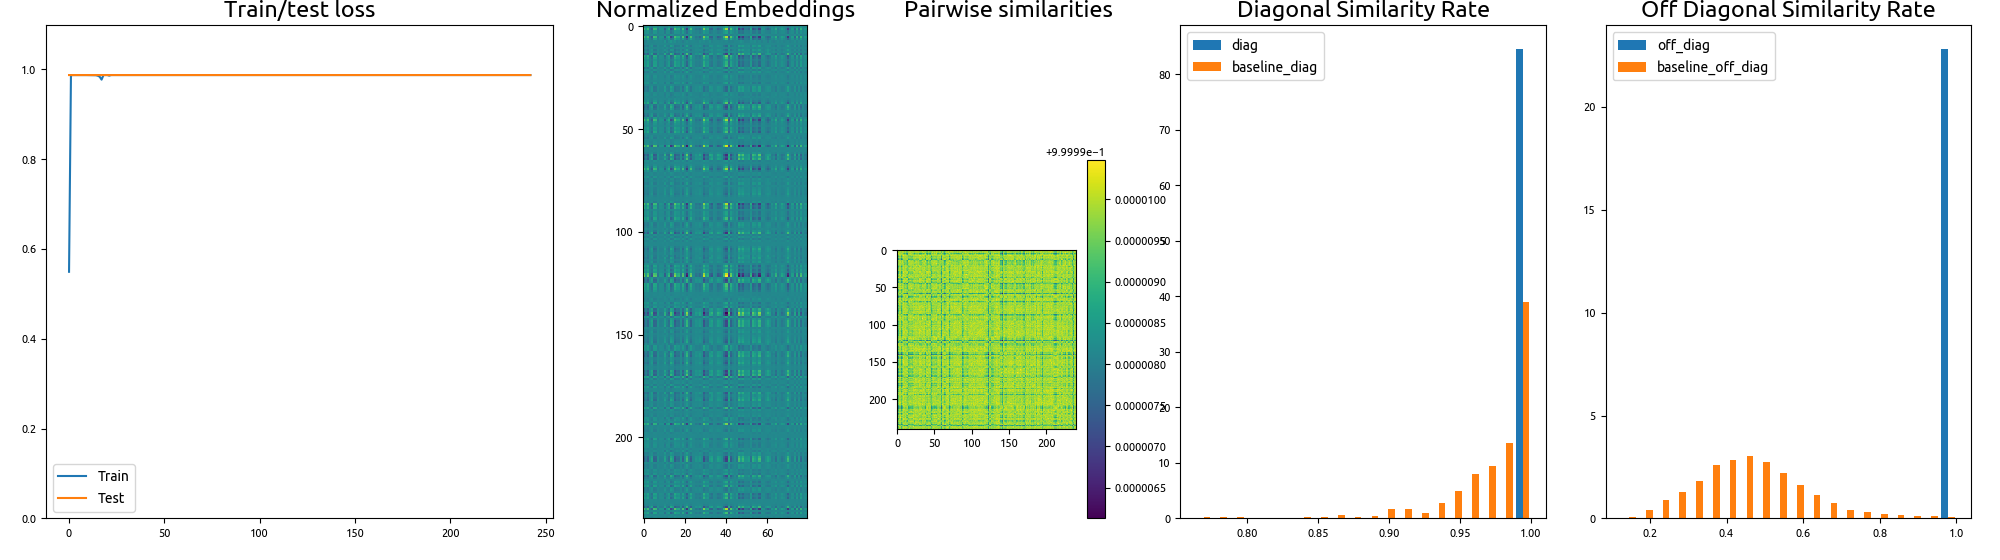
\includegraphics[width=0.9\textwidth]{figures/rome16kknn0-longskip0-lr-1e-3-0}
  \label{fig:rome16kknn0-longskip0-lr-1e-3-0-sub1}
  \caption{Sample embedding, similarity matrix, histogram, and loss curves for worst performing of this set}
\end{figure}
\begin{figure}[H]
  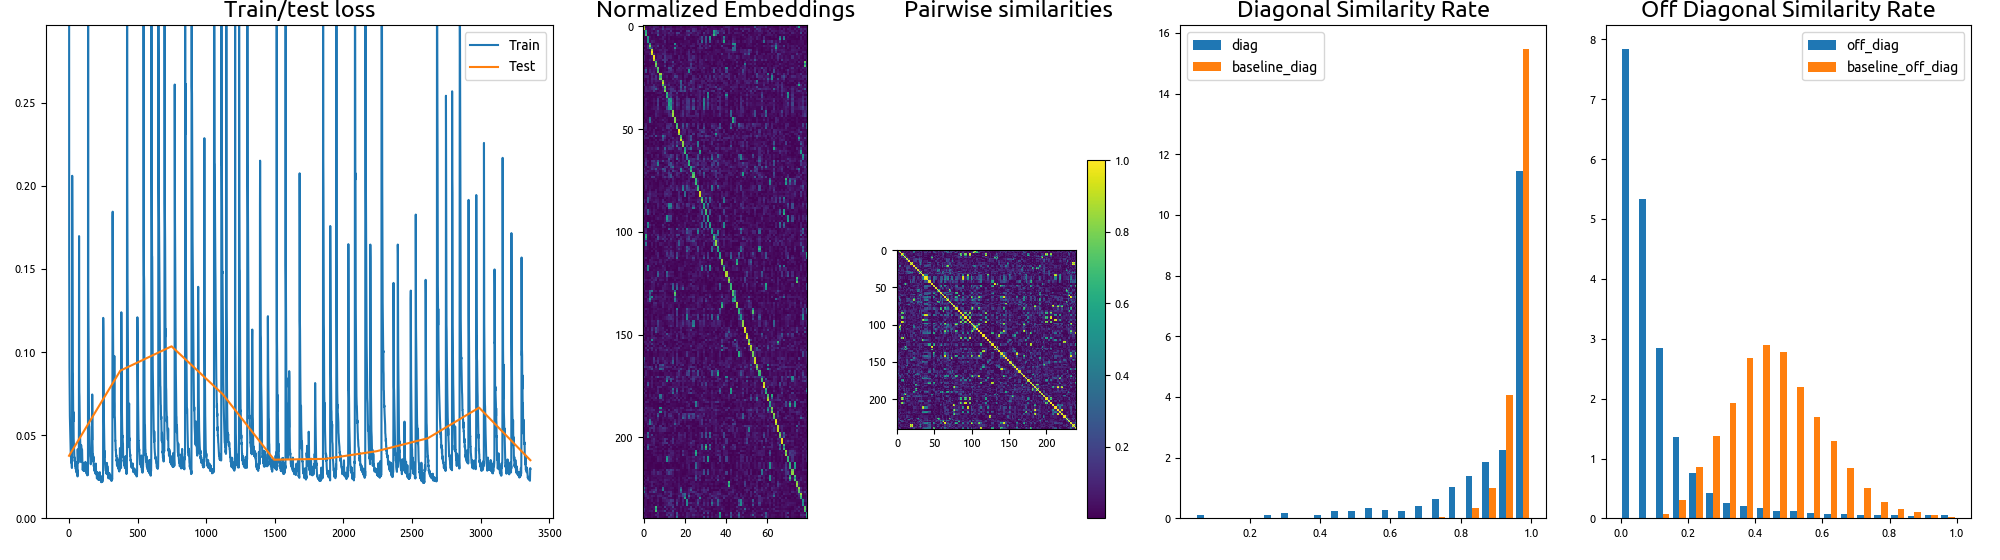
\includegraphics[width=0.9\textwidth]{figures/rome16kknn0-longskip0-lr-1e-5-0}
  \label{fig:rome16kknn0-longskip0-lr-1e-5-0-sub1}
  \caption{Sample embedding, similarity matrix, histogram, and loss curves for random experiment of this set}
\end{figure}
\begin{table}[H]
  \caption{Numerical results}
      \begin{tabular}{|l|c|c|c|} \hline
                                      &  Same Point Similarities  &  Different Point Similarities  \\ \hline
Baseline   & 9.70e-01 $\pm$ 3.84e-02 & 4.78e-01 $\pm$ 1.42e-01 \\ \hline
Long Skip Type 0 Architecture, Learning rate 1e-3   & 1.00e+00 $\pm$ 1.80e-07 & 1.00e+00 $\pm$ 4.03e-07 \\ \hline
Long Skip Type 0 Architecture, Learning rate 1e-4   & 9.00e-01 $\pm$ 1.55e-01 & 1.09e-01 $\pm$ 1.42e-01 \\ \hline
Long Skip Type 0 Architecture, Learning rate 1e-5   & 7.59e-01 $\pm$ 2.86e-01 & 7.95e-02 $\pm$ 1.19e-01 \\ \hline
      \end{tabular}
      \label{fig:tab1}
\end{table}

\subsubsection*{Rome16K Experiments Round 3}
Here I tried to use different decay rate schedules to see which worked best. All these tests used the Long Skip Type 0 Architecture and a learning rate of 1e-4. It seems exponential still works best.

\begin{figure}[H]
  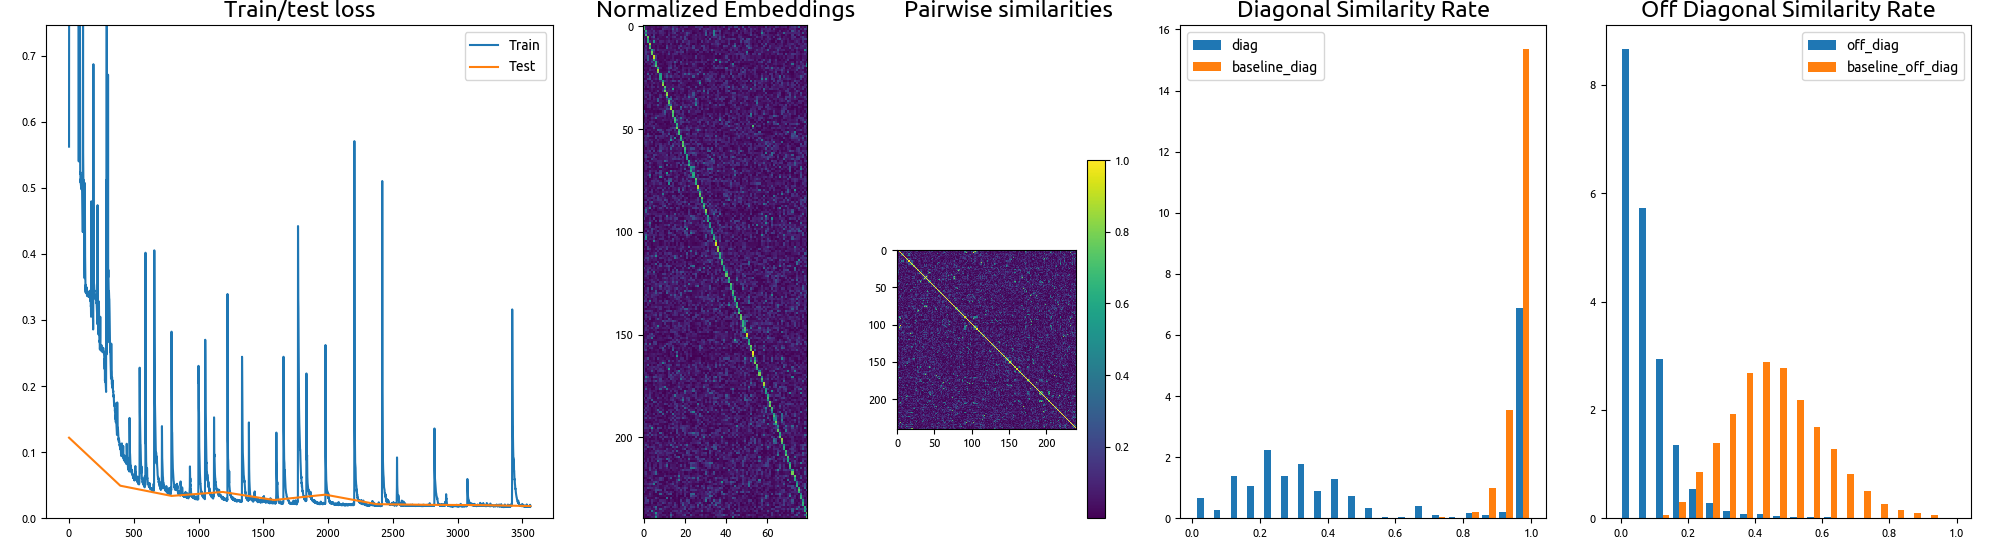
\includegraphics[width=0.9\textwidth]{figures/rome16kknn0-longskip0-lr-1e-4-type-exponential-steps-3e-1-0}
  \label{fig:rome16kknn0-longskip0-lr-1e-4-type-exponential-steps-3e-1-0-sub1}
  \caption{Sample embedding, similarity matrix, histogram, and loss curves for best performing of this set}
\end{figure}
\begin{figure}[H]
  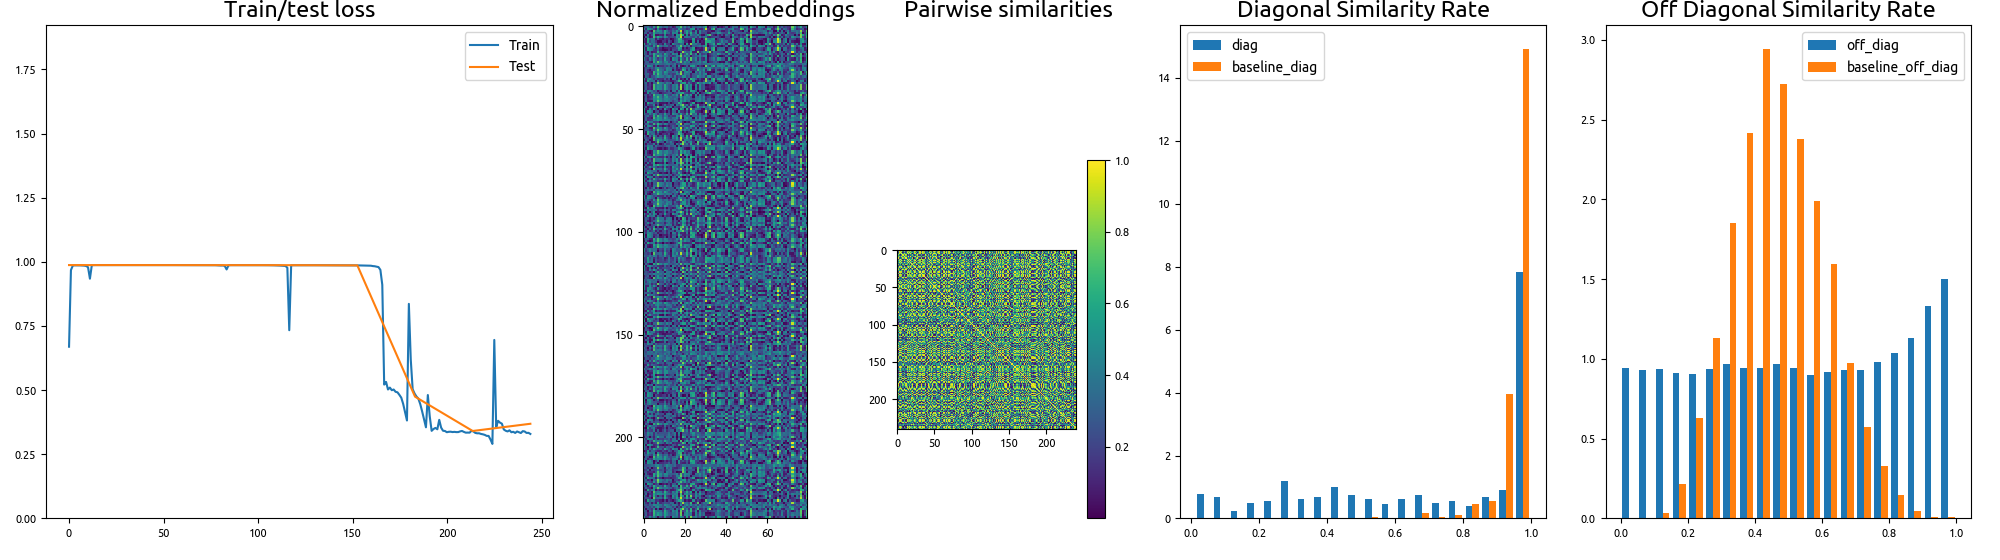
\includegraphics[width=0.9\textwidth]{figures/rome16kknn0-longskip0-lr-1e-4-type-fixed-steps-1e0-0}
  \label{fig:rome16kknn0-longskip0-lr-1e-4-type-fixed-steps-1e0-0-sub1}
  \caption{Sample embedding, similarity matrix, histogram, and loss curves for worst performing of this set}
\end{figure}
\begin{figure}[H]
  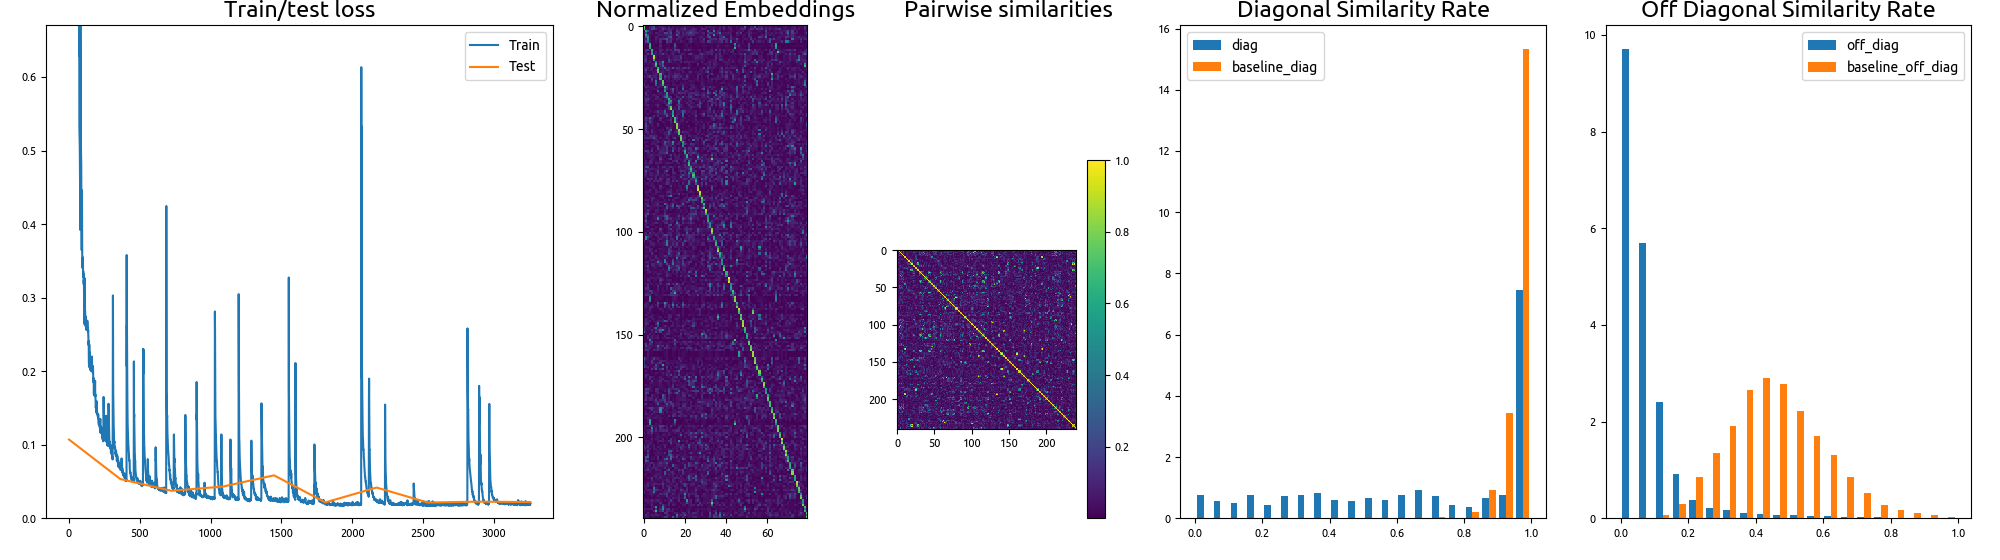
\includegraphics[width=0.9\textwidth]{figures/rome16kknn0-longskip0-lr-1e-4-type-exponential-steps-1e0-0}
  \label{fig:rome16kknn0-longskip0-lr-1e-4-type-exponential-steps-1e0-0-sub1}
  \caption{Sample embedding, similarity matrix, histogram, and loss curves for random experiment of this set}
\end{figure}
\begin{table}[H]
  \caption{Numerical results}
      \begin{tabular}{|l|c|c|c|} \hline
                                      &  Same Point Similarities  &  Different Point Similarities  \\ \hline
Baseline   & 9.70e-01 $\pm$ 3.88e-02 & 4.78e-01 $\pm$ 1.42e-01 \\ \hline
LR Decay Exponential, LR Decay Steps 1e0 & 6.94e-01 $\pm$ 3.18e-01 & 7.96e-02 $\pm$ 1.08e-01 \\ \hline
LR Decay Exponential, LR Decay Steps 3e-1& 5.84e-01 $\pm$ 3.42e-01 & 8.29e-02 $\pm$ 8.74e-02 \\ \hline
LR Decay Exponential, LR Decay Steps 5e-1& 7.66e-01 $\pm$ 2.75e-01 & 7.93e-02 $\pm$ 1.06e-01 \\ \hline
LR Decay Fixed                  & 6.69e-01 $\pm$ 3.34e-01 & 5.18e-01 $\pm$ 2.99e-01 \\ \hline
LR Decay Fixed                   & 7.84e-01 $\pm$ 2.72e-01 & 8.12e-02 $\pm$ 1.27e-01 \\ \hline
LR Decay Fixed                   & 4.64e-01 $\pm$ 4.25e-01 & 7.89e-02 $\pm$ 1.04e-01 \\ \hline
LR Decay Polynomial, LR Decay Steps 1e0  & 5.89e-01 $\pm$ 3.73e-01 & 8.11e-02 $\pm$ 1.01e-01 \\ \hline
LR Decay Polynomial, LR Decay Steps 3e-1 & 9.31e-01 $\pm$ 1.13e-01 & 1.92e-01 $\pm$ 2.06e-01 \\ \hline
LR Decay Polynomial, LR Decay Steps 5e-1 & 6.78e-01 $\pm$ 3.33e-01 & 3.18e-01 $\pm$ 2.44e-01 \\ \hline
      \end{tabular}
      \label{fig:tab1}
\end{table}


\entry{2018}{10}{08}
\subsubsection*{Rome16K Unsupervised Experiments}

\begin{figure}[H]
  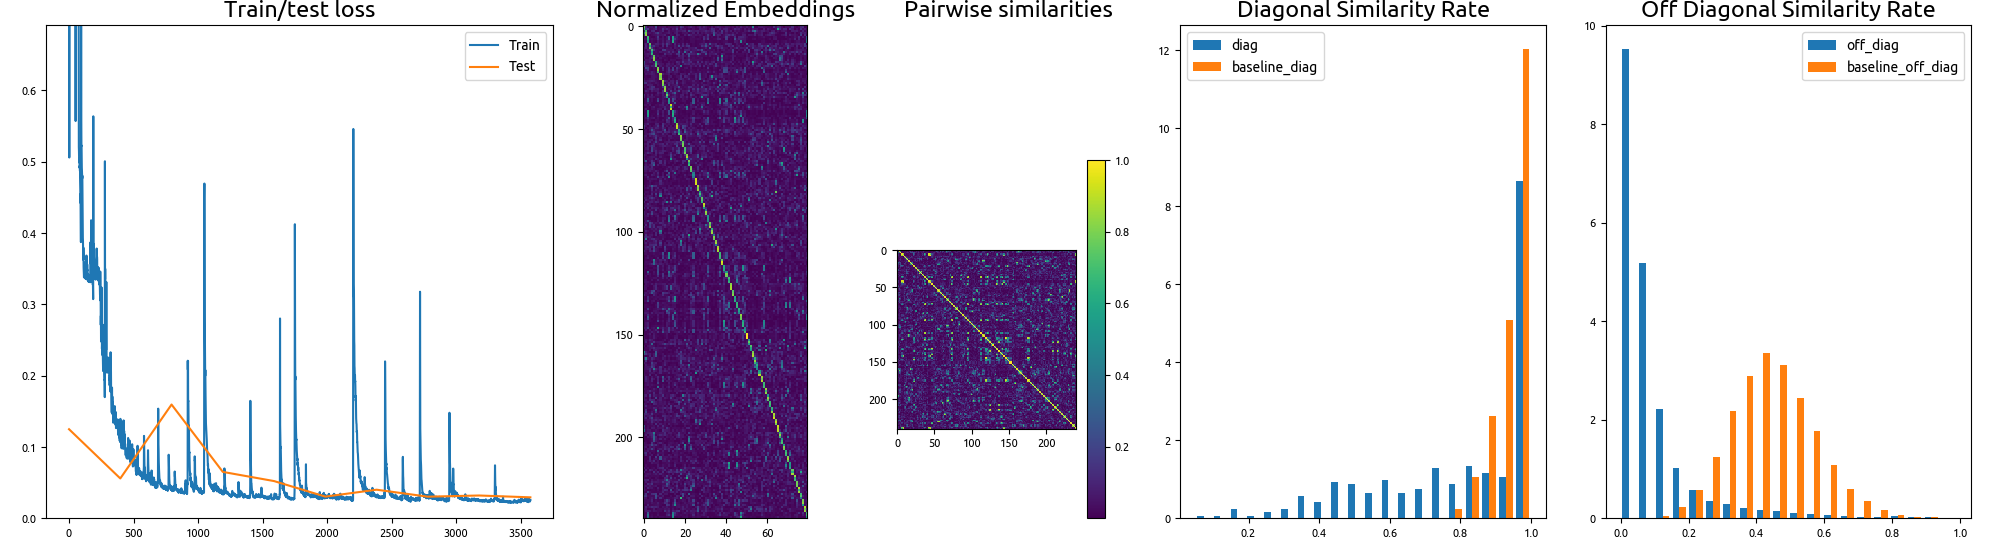
\includegraphics[width=0.9\textwidth]{figures/rome16kknn0-loss-l2-unsup-true}
  \label{fig:rome16kknn0-loss-l2-unsup-true-sub1}
  \caption{Sample embedding, similarity matrix, histogram, and loss curves for best performing of this set}
\end{figure}
\begin{figure}[H]
  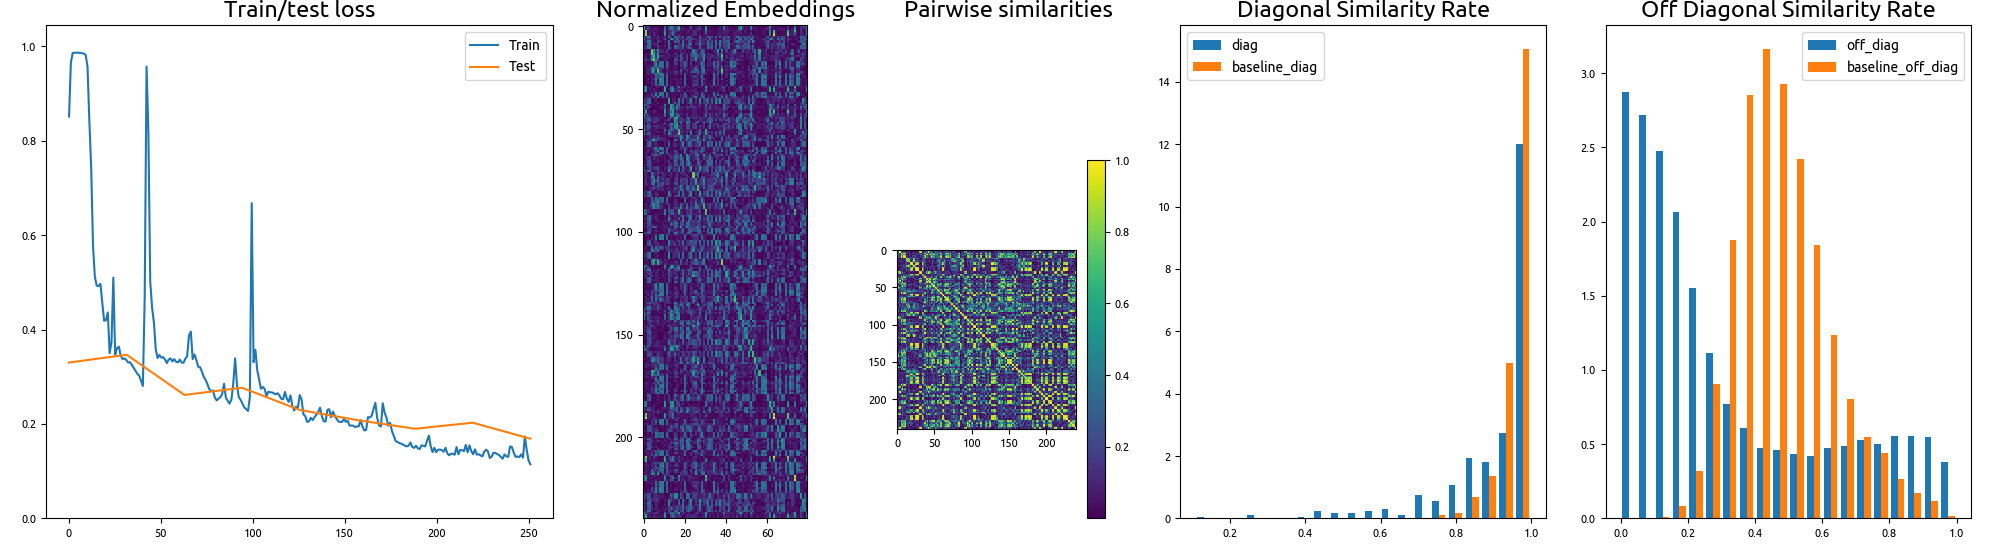
\includegraphics[width=0.9\textwidth]{figures/rome16kknn0-loss-l2-unsup-false}
  \label{fig:rome16kknn0-loss-l2-unsup-false-sub1}
  \caption{Sample embedding, similarity matrix, histogram, and loss curves for worst performing of this set}
\end{figure}
\begin{figure}[H]
  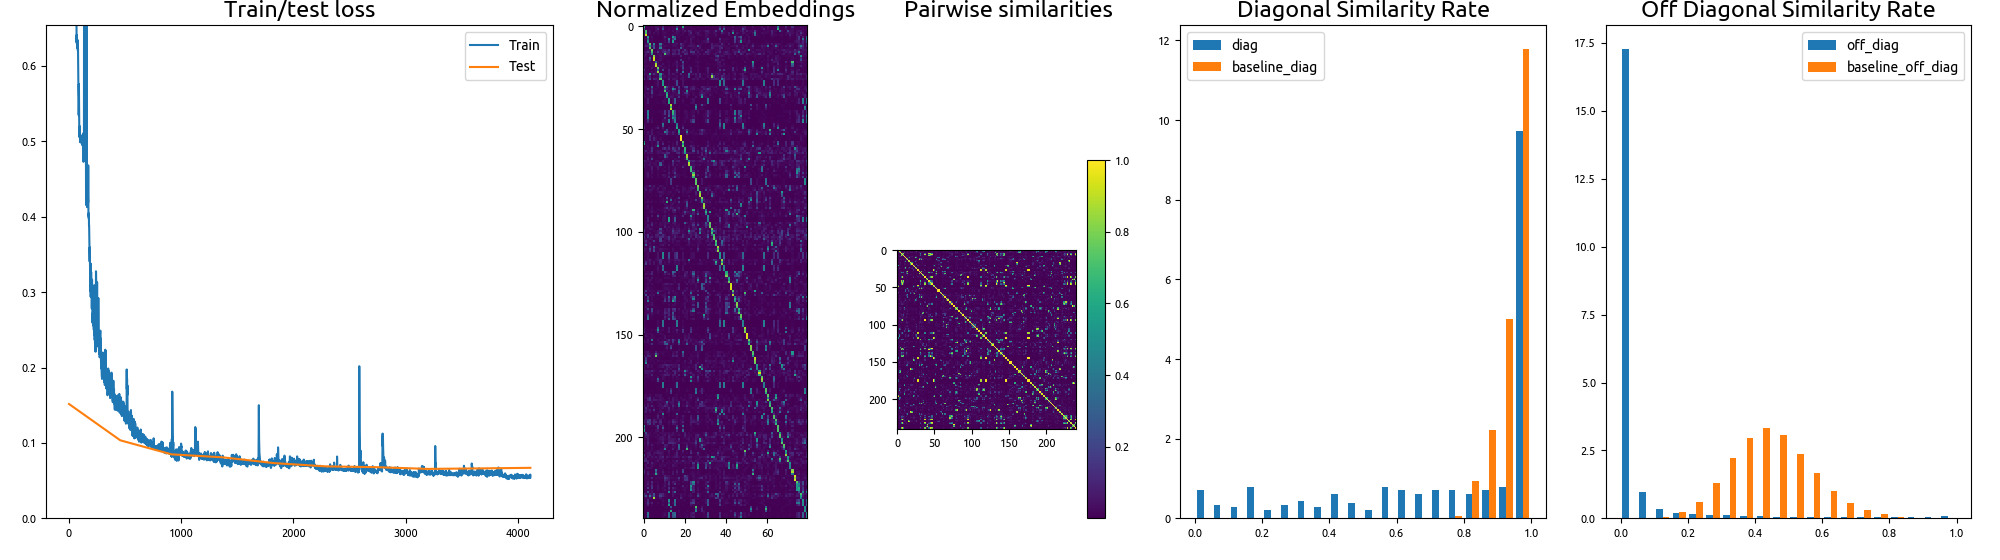
\includegraphics[width=0.9\textwidth]{figures/rome16kknn0-loss-l1-unsup-true}
  \label{fig:rome16kknn0-loss-l1-unsup-true-sub1}
  \caption{Sample embedding, similarity matrix, histogram, and loss curves for random experiment of this set}
\end{figure}
\begin{table}[H]
  \caption{Numerical results}
      \begin{tabular}{|l|c|c|c|} \hline
                                      &  Same Point Similarities  &  Different Point Similarities  \\ \hline
Baseline   & 8.83e-01 $\pm$ 1.26e-01 & 4.67e-01 $\pm$ 1.32e-01 \\ \hline
Data type \texttt{rome16kknn0}, Loss L1, Supervised   & 5.62e-01 $\pm$ 4.12e-01 & 4.63e-02 $\pm$ 1.31e-01 \\ \hline
Data type \texttt{rome16kknn0}, Loss L1, Unsupervised   & 6.89e-01 $\pm$ 3.50e-01 & 5.79e-02 $\pm$ 1.62e-01 \\ \hline
Data type \texttt{rome16kknn0}, Loss L2, Supervised   & 7.84e-01 $\pm$ 2.54e-01 & 3.16e-01 $\pm$ 2.74e-01 \\ \hline
Data type \texttt{rome16kknn0}, Loss L2, Unsupervised   & 7.21e-01 $\pm$ 2.88e-01 & 1.09e-01 $\pm$ 1.45e-01 \\ \hline
      \end{tabular}
      \label{fig:tab1}
\end{table}



\end{document}






